\documentclass[%
 reprint,
%superscriptaddress,
%groupedaddress,
%unsortedaddress,
%runinaddress,
%frontmatterverbose, 
%preprint,
%showpacs,preprintnumbers,
%nofootinbib,
%nobibnotes,
%bibnotes,
 amsmath,amssymb,
 aps,
%pra,
%prb,
%rmp,
prstab,
%prstper,
%floatfix,
longbibliography
]{revtex4-1}

\usepackage{graphicx}% Include figure files
\usepackage{dcolumn}% Align table columns on decimal point
\usepackage{bm}% bold math
\usepackage{hyperref}% add hypertext capabilities
%\usepackage[mathlines]{lineno}% Enable numbering of text and display math
%\linenumbers\relax % Commence numbering lines
\usepackage{color}
%\usepackage{siunitx}
\usepackage{url}

%\usepackage[showframe,%Uncomment any one of the following lines to test 
%%scale=0.7, marginratio={1:1, 2:3}, ignoreall,% default settings
%%text={7in,10in},centering,
%%margin=1.5in,
%%total={6.5in,8.75in}, top=1.2in, left=0.9in, includefoot,
%%height=10in,a5paper,hmargin={3cm,0.8in},
%]{geometry}

\DeclareFontFamily{U}{wncy}{}
\DeclareFontShape{U}{wncy}{m}{n}{<->wncyr10}{}
\DeclareSymbolFont{mcy}{U}{wncy}{m}{n}
\DeclareMathSymbol{\Sh}{\mathord}{mcy}{"58} 

\newcommand{\q}[2]{\ensuremath{#1\ \mathrm{#2}}} % quantity with units

\begin{document}

\title{Experimental and numerical studies of the effects of resonant
  and random excitations of the proton beam in the LHC, with
  applications to the design of a pulsed hollow electron lens for
  active halo control}

\thanks{Fermilab is operated by Fermi Research Alliance, LLC under
	Contract No.~DE-AC02-07CH11359 with the United States Department of
	Energy. This work was partially supported by the US DOE LHC
	Accelerator Research Program (LARP) and by the European FP7 HiLumi
	LHC Design Study, Grant Agreement 284404.}

\author{Miriam Fitterer}
 \email{mfittere@fnal.gov}
\author{Giulio Stancari}
\author{Alexander Valishev}
\affiliation{Fermi National Accelerator Laboratory, Batavia, Illinois, USA}

\author{Stefano Redaelli}
\author{Daniel Valuch}
\affiliation{CERN, Geneva, Switzerland}

\date{\today}

\begin{abstract}
  In the High Luminosity Large Hadron Collider (HL-LHC), a
  considerable amount of energy will be stored in the beam tails, due
  to the high beam intensity and to an overpopulation of the tails
  compared to a Gaussian distribution. To control and clean the beam
  halo, the installation of two hollow electron lenses (HEL), one per
  beam, is being considered. In standard electron-lens operation, a
  proton bunch sees the same electron current at every
  revolution. Pulsed operation (i.e., different current for different
  turns) is also considered, because it can widen the range of
  achievable halo removal rates. For an axially symmetric electron
  lens, only the halo particles are excited, leaving the core
  unperturbed. If a residual field is present at the location of the
  beam core, these particles are exposed to transverse kicks and to
  noise. In this paper, we present the results of numerical
  simulations and of the LHC experiments conducted in~2016 and~2017 to
  study the effects of random noise and of resonant excitations on the
  beam core. The excitation patterns were generated by the transverse
  damper system, which is a very flexible source of transverse dipole
  kicks. The main observables were losses, emittances, and transverse
  distributions as a function of excitation patterns and
  strengths. The resonant excitations showed rich nonlinear dynamics
  and nontrivial changes of the beam distribution, which, to our
  knowledge, have not previously been observed and studied in this
  detail. We also give estimates, based upon existing measurements of
  prototype electron guns, of the residual fields that may be expected
  in the HL-LHC hollow electron lens.
\end{abstract}

% PACS 2008:
% 29.20.db Storage rings and colliders

\pacs{29.20.D-}% PACS, the Physics and Astrtheonomy
                             % Classification Scheme.
%\keywords{Suggested keywords}%Use showkeys class option if keyword
                              %display desired
\maketitle

%\tableofcontents

\section{Introduction}
\label{sec:intro}

\begin{table*}
  \caption{ Stored beam energy for different past, present and future
    colliders. Each new machine represents a leap in stored beam
    energy.}
  \label{tab:stored_energy}
  \begin{ruledtabular}
    \begin{tabular}{lccccc}
      Collider& Tevatron (protons) \cite{tevatron} & LHC 2016 \cite{chamonix2017param}	& LHC nominal \cite{lhc_design} & HL-LHC \cite{hlcdr} & FCC \cite{fcc_param_2017} \\
      \colrule
      Beam energy [TeV] & 0.98 & 6.5 & 7.0 & 7.0 & 50.0\\
      Number of bunches & 36 & 2220 & 2808 & 2748 & ? \\
      Number of particles per bunch & $2.90\times 10^{11}$ & $1.15\times 10^{11}$ & $1.15\times 10^{11}$ & $2.2\times 10^{11}$ & $1.0\times 10^{11}$\\
      Stored beam energy [MJ] & 1.6 & 265.9 & 362.2 & 678.0 & 8400 \\
    \end{tabular}
  \end{ruledtabular}
\end{table*}
      
\begin{figure*}
  \begin{minipage}[c]{\columnwidth}
    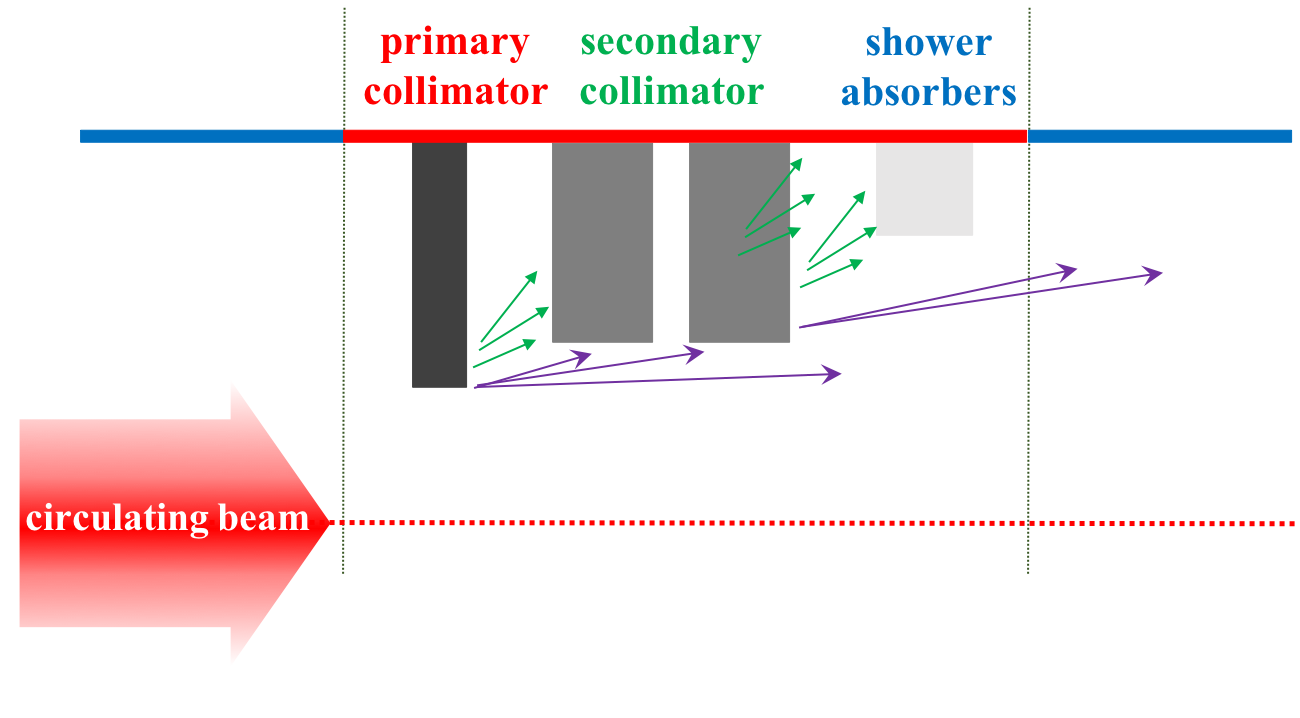
\includegraphics[width=\columnwidth]{passive_halo_control.png}
    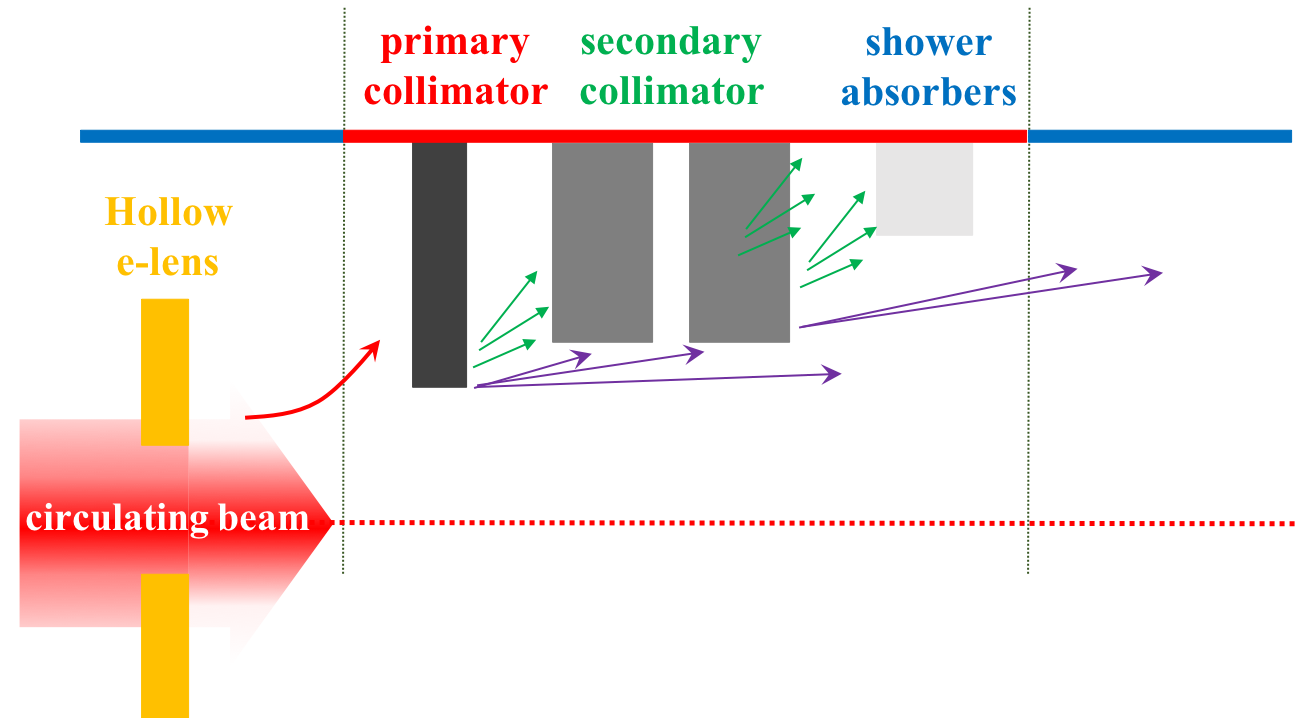
\includegraphics[width=\columnwidth]{active_halo_control.png}
  \end{minipage}
  \hfill
  \begin{minipage}[c]{\columnwidth}
  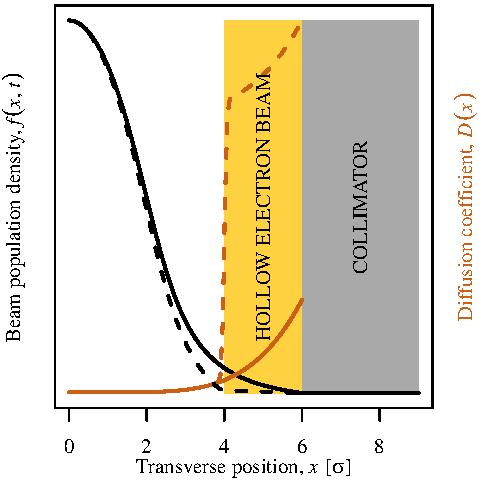
\includegraphics[width=\columnwidth]{diffusion_illustration}
  \end{minipage}
  \caption{Left: Sketch of passive halo control with a conventional
    collimation system (top) and active halo control, with the
    addition of a hollow electron lens (bottom). Right: Illustration
    of a simplified model of active diffusion enhancement in the
    transverse plane. The diffusion coefficient as a function of
    amplitude (orange) is enhanced in a specific amplitude region when
    the hollow beam is turned on (from solid to dashed line). A
    corresponding reduction in beam tail population (black) is created
    (from solid to dashed line).}
  \label{fig:active_halo_control} 
\end{figure*}

Considering past, current and future high energy colliders, each new
machine has represented a considerable leap in stored beam energy
(Table~\ref{tab:stored_energy}).

Furthermore, recent measurements at the LHC show that the tails of the
transverse beam distribution are overpopulated compared to a Gaussian
distribution. This results in a considerable amount of energy being
stored in the beam tails. In particular, in the case of the LHC, about
5\% of the beam population is stored in the tails (i.e., above
3.5$\sigma$, where $\sigma$ is the Gaussian rms core beam size),
compared to 0.22\% in an ideal Gaussian distribution, leading to 19~MJ
of stored energy for nominal LHC parameters and 34~MJ in the case of
HL-LHC~\cite{helreview_valentino}. This leads to the conclusion that a
mechanism is needed to deplete the beam tails in a controlled
manner. Further information on the needs for halo control in LHC can
be found in Ref.~\cite{helreview}.

The most direct approach is to decrease the collimator gaps or to
periodically scrape the tails. However, this is not feasible, as it
would generate unacceptably large loss spikes and possibly component
damage. Most promising are methods which increase the diffusion speed
in the region of the halo particles, resulting in a smooth and
continuous removal of the high amplitude tails, while leaving the core
of the beam unperturbed. The diffusing halo particles are then
intercepted by the collimation system and removed. This concept is
also referred to as active halo control, designed to enhance a
conventional passive system, which is still needed to robustly
intercept the halo particles. An illustration of the concept is shown
in Fig.~\ref{fig:active_halo_control}.

In a recent review, the need for such an active halo control system
for HL-LHC has been assessed, with the conclusion that it would
considerably increase the operational margins and reduce the risks for
machine protection~\cite{helreview}. In view of the need of active
halo control for HL-LHC and for future high power accelerators, like
HE-LHC and FCC-hh~\cite{helhcparam2011, fcc_coll_ipac2017}, different
active halo control methods have been
studied~\cite{helreview_bruce}. The hollow electron lens (HEL) is
considered the most established, flexible and suitable technology for
the HL-LHC~\cite{hel_tevatron_stancari, helreview}.

However, the beneficial effects of an HL-LHC HEL for machine
protection and for collimation cannot come at the expense of
performance degradation due to losses or emittance growth in the beam
core. In standard electron-lens operation, a proton bunch sees the
same electron current at every revolution. It is also possible to have
different currents for different groups of bunches. Under these
conditions, the imperfections of the hollow beam have a negligible
effect. On the other hand, in order to extend the range of achievable
removal rates, pulsed operation is also being considered. In this
case, different currents can be set to act on the same bunch at each
turn. If a residual field is present at the location of the beam core,
core particles can be exposed to resonant transverse kicks and to
noise.

In this paper, we concentrate on the experimental and numerical
assessment of possible detrimental effects on the beam core of a
pulsed electron lens. Section~\ref{sec:hel} gives an introduction to
the concept of HELs and summarizes the design parameters of the HL-LHC
HELs. Section~\ref{sec:core} is dedicated to the sources of residual
fields from the HEL in the core region. Sections~\ref{sec:exp}
and~\ref{sec:sim} describe the experimental conditions and the setup
of the numerical tracking simulations. Results and comparisons between
simulations and measurements are given in Section~\ref{sec:simex},
with discussion and summary in Section~\ref{sec:sum}. Auxiliary data
and plots are collected in the Appendices.



\section{Hollow electron lens for HL-LHC}
\label{sec:hel}

\begin{figure*}
  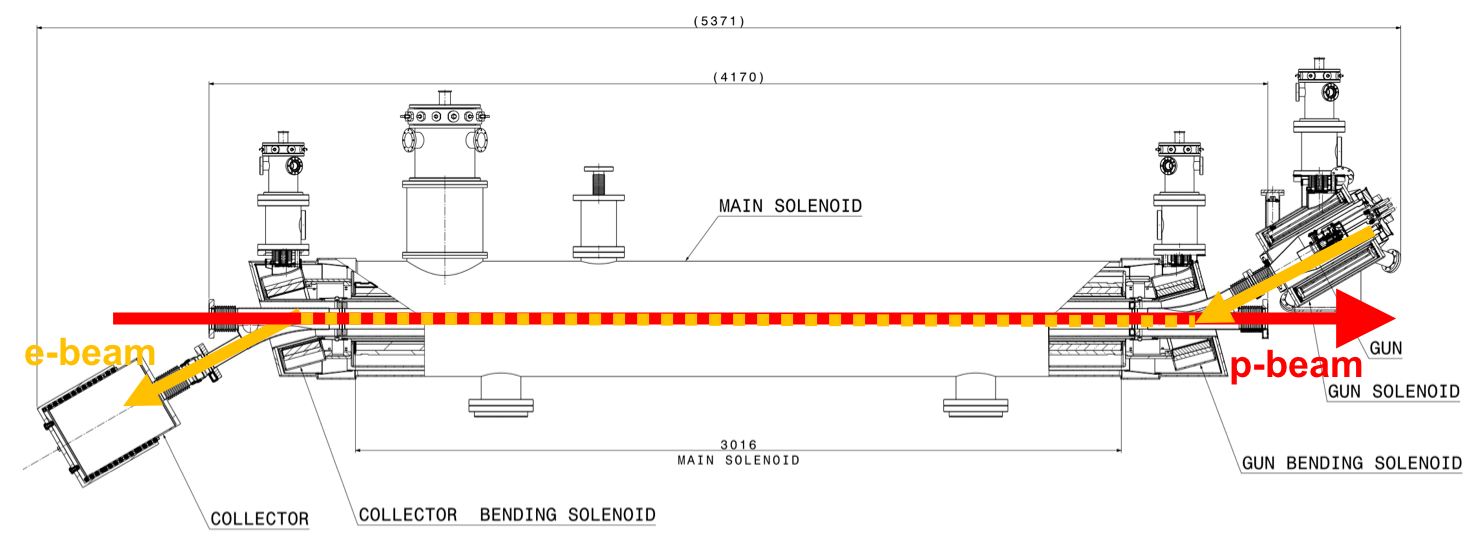
\includegraphics[width=0.75\textwidth]{hel_layout_epbeam}
  \caption{Layout of the hollow electron lens for HL-LHC. (Courtesy of
    CERN EN-MME mechanical engineering group.)}
  \label{fig:hel_layout}
\end{figure*}

\begin{figure}
  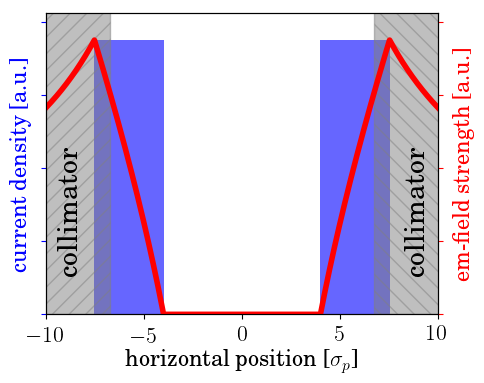
\includegraphics[width=0.8\columnwidth]{kick_hel_lhc_no_grid}
  \caption{Illustration of the hollow electron beam charge
    distribution (blue), of the magnitude of the transverse kick
    experienced by the proton beam (red), and of the position of the
    primary collimators (gray).}
  \label{fig:hel_field}
\end{figure}

\begin{table}
  \caption{HL-LHC design parameters at top energy~\cite{hlcdr} and
    parameters relevant to the HEL. Optics parameters at the HEL are
    based on a position of $-$40~m for Beam~1 (B1) and $+$40~m for
    Beam~2 (B2) from the interaction point IP4, using HL-LHC optics
    V1.3 with $\beta^{*} = \q{0.15}{m}$~\cite{hlv13}.}
  \label{tab:hllhc_param}
  \begin{ruledtabular}
    \begin{tabular}{lccc}
      Beam parameters & \multicolumn{2}{c}{Value} & Unit\\
                       & B1 & B2 & \\
      \colrule
      Beam energy,  $E_{p}$  &  \multicolumn{2}{c}{7} & TeV\\
      Number of bunches, $n_b$ & \multicolumn{2}{c}{2748} &  \\
      Bunch population, $N_b$ & \multicolumn{2}{c}{$2.2\times 10^{11}$} & \\
      Normalized emittance, $\epsilon_{N,x/y}$ & \multicolumn{2}{c}{2.5} & $\mu$m\\
      Bunch spacing & \multicolumn{2}{c}{25} & ns\\
      \colrule
      \multicolumn{4}{l}{Optics parameters at HEL (B1)\footnote{As the
      Twiss parameters at IP4 do not change during the entire squeeze
      of the optical functions, and IP4 and the HEL are only separated
      by a drift space, the Twiss parameters stay constant also at the
      HEL during the squeeze.}} \\
      \colrule
      $\beta_{x}$ at HEL  & 197.5 & 280.6 & m\\
      $\beta_{y}$ at HEL & 211.9 & 262.6 & m\\
      Dispersion $D_{x}$ at HEL & 0.0& 0.0 & m\\
      Dispersion $D_{y}$ at HEL & 0.0& 0.0 & m\\
      Proton beam size $\sigma_{p,x}$ at HEL & 0.26 & 0.31& mm \\		
      Proton beam size $\sigma_{p,y}$ at HEL & 0.27 & 0.30 &mm \\
      \multicolumn{4}{l}{Scale of scraping positions}\\ \hspace{6ex}$\sigma_{p}=\max(\sigma_{p,x},\sigma_{p,y})$ & 0.27& 0.31 & mm\\
    \end{tabular}
  \end{ruledtabular}
\end{table}

\begin{table}
  \caption{HL-LHC hollow electron lens parameters, as defined in
    Ref.~\cite{hel_cdr}.}
  \label{tab:hel_param}
  \begin{ruledtabular}
    \begin{tabular}{lcc}
      Geometry & Value& Unit\\
      \colrule
      Length, $L$    &  3 & m\\
      % 3-8 sigmap with 3.5 um -> 3.55-9.47 for 2.5 um emittance
      Desired range of scraping positions & 3.5--9.5 &$\sigma_p$\\
      \colrule
      Magnetic fields & & \\
      \colrule
      Gun solenoid, $B_g$ & 0.2--0.4 & T\\
      Main solenoid, $B_m$ & 2--6 & T\\
      Collector solenoid, $B_c$ & 0.2--0.4 & T\\
      Compression factor, $k \equiv \sqrt{B_m/B_g}$ & 2.2--5.5 &  \\
      \colrule
      Electron gun & & \\
      \colrule
      Peak yield $I_e$ at 10~keV & 5.0 & A\\
      Gun perveance, $P$ & 5 & $\mu$perv\\
      Inner/outer cathode radii, $R_1/R_2$ & 6.75/12.7 & mm\\
      \colrule
      High-voltage modulator & & \\
      \colrule
      Cathode-anode voltage & 10.0 & kV\\
      Rise time (10\%-90\%) & 200 & ns \\
      Repetition rate & 35 & kHz
    \end{tabular}
  \end{ruledtabular}
\end{table}


\subsection{General overview}
\label{sec:hel:intro}

Electron lenses are based upon continuous or pulsed low-energy,
magnetically confined electron beams~\cite{Shiltsev:PRSTAB:2008,
  Fischer:PRL:2015, Shiltsev:elens-book:2016}. The electron beam is
generated in an electron gun, guided and confined by strong solenoids
and finally dumped in a collector. As an example, the conceptual
design of the HL-LHC HEL is shown in Fig.~\ref{fig:hel_layout}.

The circulating beam (protons in the LHC case) is affected by the
electromagnetic field of the electron beam. For the application of
active halo control, the electron beam needs to generate an
electromagnetic field only at the location of the halo particles. This
field distribution can be achieved, for instance, by using a hollow
charge distribution in radius $r=\sqrt{x^2+y^2}$, uniformly
distributed between inner radius $R_1$ and outer radius $R_2$
(Fig.~\ref{fig:hel_field}). In this case, the circulating proton beam
experiences the following radial kick $\theta(r)$:
%
\begin{equation}
  \label{eq:field_1}
  \theta(r)=\frac{f(r)}{(r/R_2)}\cdot \theta_{\rm max},
\end{equation}
%
where $f(r)$ is a shape function with
%
\begin{equation}
  \label{eq:field_2}
  f(r) =
  \begin{cases}
    0 &,\quad r< R_1,\\
    \frac{r^2-R_1^2}{R_2^2-R_1^2} &,\quad R_1 \leq r < R_2,\\
    1 &,\quad R_2 \leq r
  \end{cases}
\end{equation}
%
and $\theta_{\rm max}=\theta(R_2)$ is the maximum kick angle given by
%
\begin{equation}
  \label{hel_kick_max}
  \theta_{\rm max} = \theta(R_2) =
  \frac{2LI_T(1\pm\beta_e\beta_p)}{4\pi\epsilon_0  \cdot
    \left(p_0/q\right)_p \cdot \beta_e\beta_p
    c^2}\cdot\frac{1}{R_2},
\end{equation}
%
with $L$ the length of the HEL, $I_T$ the total electron beam current,
$\beta_{e}$ and $\beta_{p}$ the relativistic velocity parameters of
electrons and protons, $\left(p_0/q\right)_p = \left(B\rho\right)_p$
the magnetic rigidity for the proton beam reference particle, $c$ the
speed of light and $\epsilon_0$ the vacuum permittivity. The
$\pm$-sign in Eq.~\ref{hel_kick_max} represents the two cases of the
electron beam traveling in the direction of the proton beam
($v_e v_p>0$) leading to ``$-$" or in the opposite direction
($v_e v_p<0$) leading to ``$+$". For hollow electron beam collimation,
electrons and protons are chosen to counterrotate, so that the
magnetic and electric kicks add up. (For simplicity, the dependence of
the electron axial velocity on radius is neglected in
Eq.~\ref{hel_kick_max}.)

In the case of HL-LHC HEL design parameters
(Table~\ref{tab:hllhc_param} and Table~\ref{tab:hel_param}), the
maximum kick is:
%
\begin{equation}
  \label{eqn:helkick}
  \theta_{\rm max,B1} = 392~\rm{nrad}
\end{equation}
%
for an inner radius of $R_1 = 4\sigma_p$, outer radius $R_2 =
7.5\sigma_p$, peak current of $I_e = \q{5.0}{A}$, using the Beam~1
lattice of the LHC. Similar values are obtained for Beam~2.


\subsection{Operation modes and effects on the beam core}
\label{sec:hel:core}

For the HEL, two modes of operation are currently under consideration:
the continuous mode (also referred to as `DC', or direct current, in
this paper) as standard operation mode, described above; and the
pulsed mode. The main benefit of pulsed HEL operation is the increase
in halo removal rates. A wider range of removal rates may become
important under operating conditions with small nonlinearities, in
particular low chromaticity and octupole current, when the DC mode may
be too slow~\cite{hel_halo_hllhc_fitterer, hl_halo_ipac2017}.

Two different pulsing patterns are considered for the HL-LHC. In both
cases, at each passage, a given bunch sees a different electron-lens
current and, therefore, experiences a different transverse kick. The
patterns are defined as follows:

\begin{itemize}

\item \textbf{random excitation:} The extraction voltage in the
  electron gun is modulated according to the
  following expression:
%
  \begin{equation}
    U_{\mathrm{e-gun}} = (1-a) \cdot U_{\mathrm{max}} +
    a \cdot \eta \cdot U_{\mathrm{max}},
  \end{equation}
%
  where $U_{\mathrm{max}}$ is the maximum voltage, $a$ is the
  modulation strength, with $a \in [0,1]$, and $\eta$ is a uniformly
  distributed random number in the interval~$[0,1]$. Simulations and
  experiments, discussed below, were usually conducted with $a = 1$.

\item \textbf{resonant excitation:} The electron beam is switched on
  only every $k^{\mathrm{th}}$ turn. The excitation can be represented
  by the following expression:
  \begin{eqnarray}
    \label{intro:eqn:1}
    f(t) & = & \sum_{n=-\infty}^{+\infty}\delta\left[t-n\cdot(kT)\right],
  \end{eqnarray}
  where $n$ is the turn number and $T$ is the revolution period. Its
  Fourier representation is
  \begin{equation}
    \label{intro:eqn:2}
    f(t) = \Sh_{kT}(t) = \frac{1}{kT}\sum_{n=-\infty}^{+\infty}e^{2\pi i f_nt},
  \end{equation}
  with $f_n = n \cdot f_{\rm rev} / k$ and
  where $\Sh_{kT}$ is the Dirac comb. In general,
  $k^{\mathrm{th}}$~turn pulsing drives $k^{\mathrm{th}}$-order
  resonances~\cite{md_sim_hel_res_ex_fitterer}. This type of pulsing
  pattern was used in the Tevatron during regular collider operations
  for abort-gap cleaning~\cite{hel_tevatron_abortgap_zhang}.
\end{itemize}

For an axially symmetric electron lens, the field at the beam core
vanishes. Effects on the proton core arise from imperfections, with
two main sources: the injection and extraction bends of the HEL
(discussed below in Section~\ref{core:sec:1}), where the electron beam
crosses the proton beam; and distortions of the electron beam profile
during its propagation under magnetic focusing and space charge
(Section~\ref{core:sec:2}). Both sources result in nonlinear
kicks~\cite{hel_bends_stancari, hel_model_polynomial_morozov}. In
continuous operation, these nonlinear kicks are usually much smaller
than the machine nonlinearities. Tolerances on imperfections are
therefore not particularly stringent. The picture changes
significantly in case of pulsed operation. If the electromagnetic
field does not vanish at the proton beam core, noise or resonant kicks
are transferred not only to the halo particles, as intended, but also
to the beam core. Tolerances on the residual fields in this case
become much more stringent. Studies of the effects of the HEL on the
beam core therefore focus on this mode of operation, which is also the
main subject of this paper.



\section{Sources and estimates of residual fields}
\label{sec:core}

\begin{figure*}
  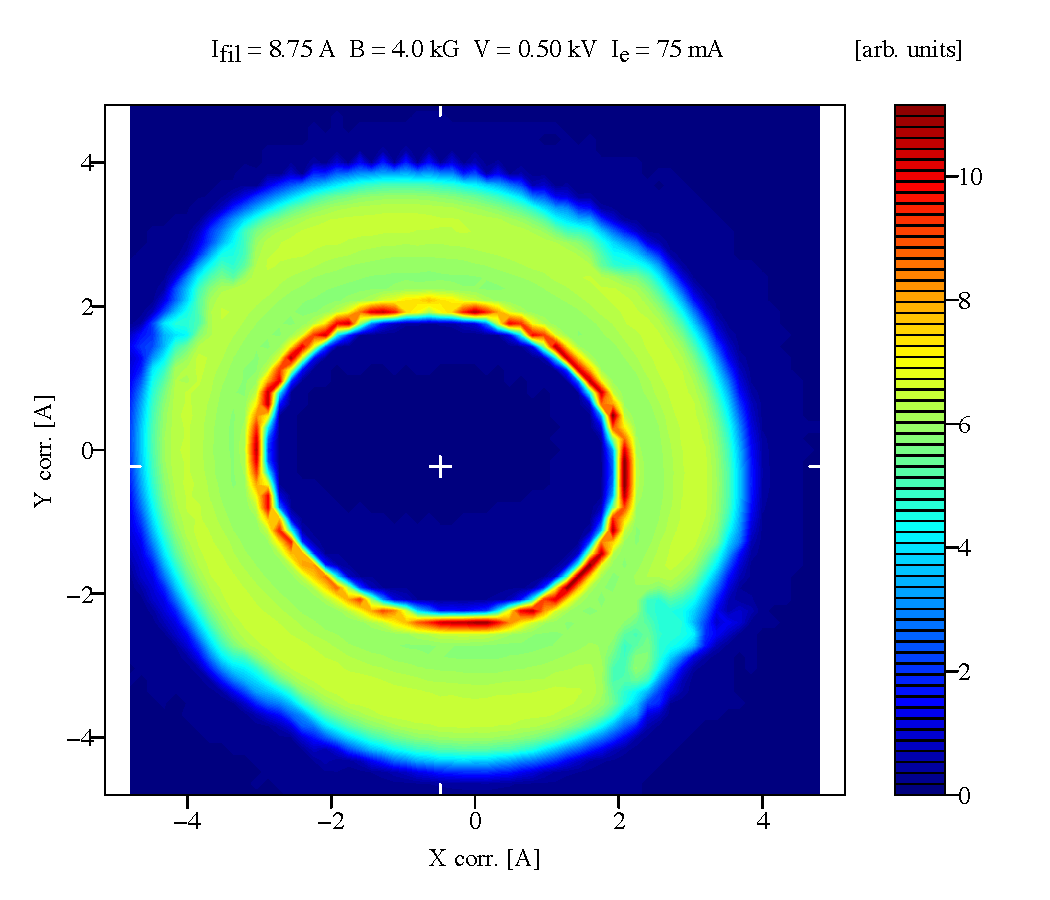
\includegraphics[height=0.9\columnwidth]{CHG1b_170523_8p75A_2-4-2kG_500V_75mA_hires_2D} \hfill
  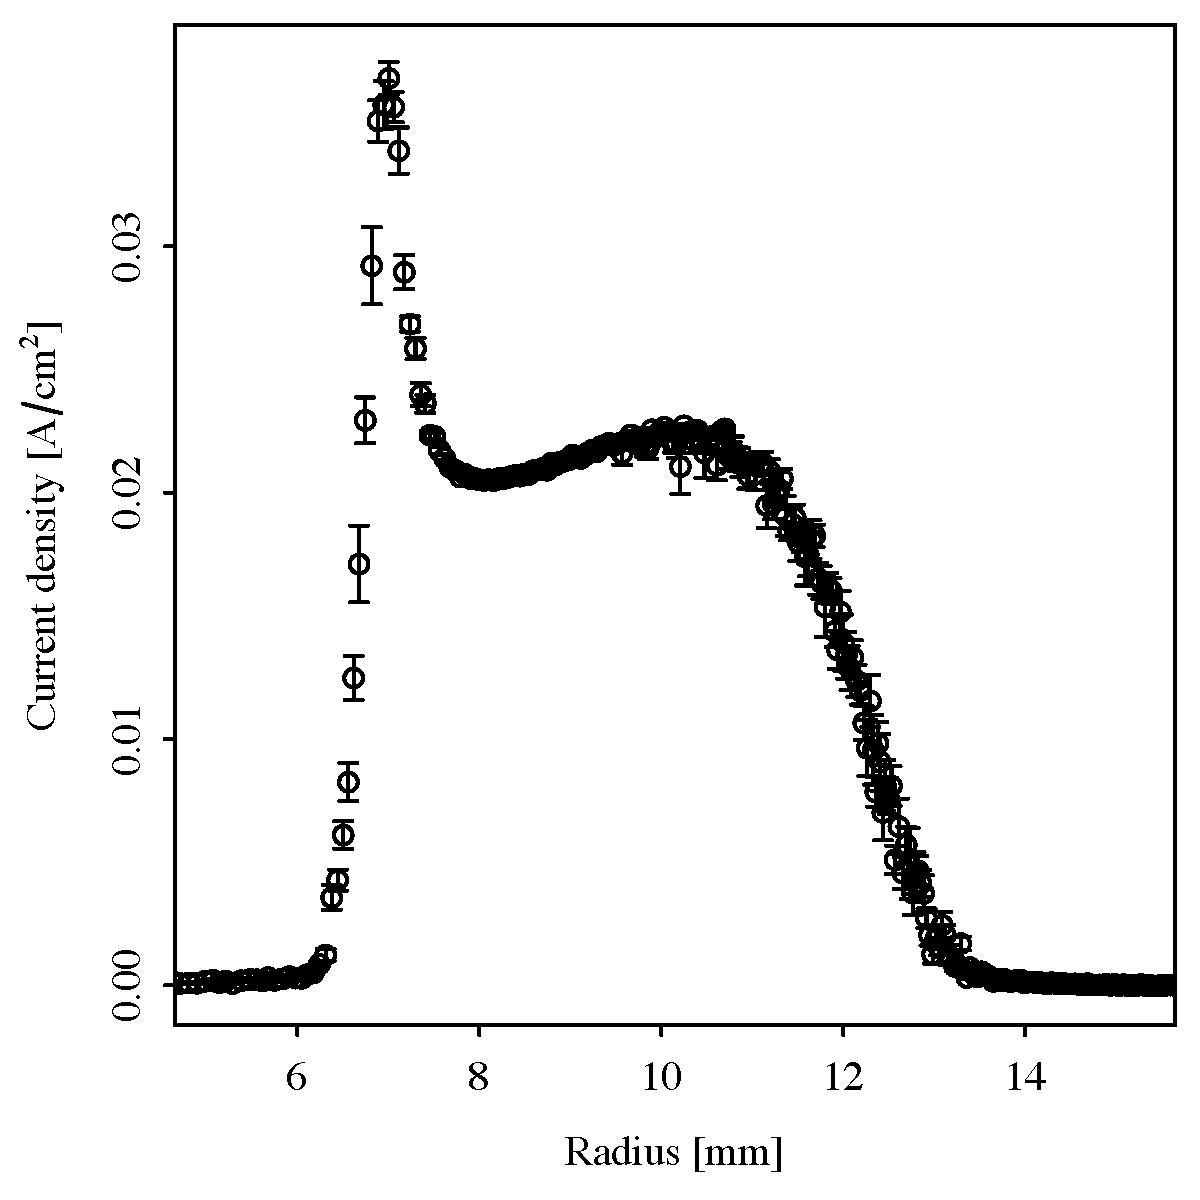
\includegraphics[height=0.9\columnwidth]{CHG1b_170523_8p75A_2-4-2kG_500V_75mA_hires_j-vs-r_binned_nogrid_nolabel}
  \caption{Example of current-density distribution measurements for
    the hollow electron gun prototype CHG1b, taken at the Fermilab
    electron lens test stand in
    2017~\cite{hel_res_field_stancari_2017}: 2-dimensional transverse
    profile measurement (left) and calculated 1-dimensional radial
    projection (right).}
  \label{core:fig:0}
\end{figure*}

\begin{figure*}
  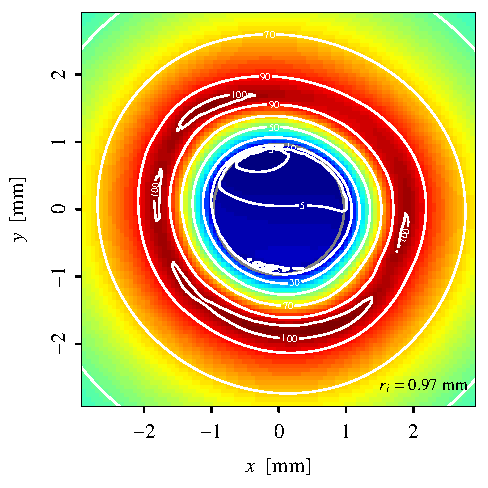
\includegraphics[width=\columnwidth]{CHG1b_170512_8p75A_2-4-2p7kG_500V_76mA_hires_Emap} \hfill
  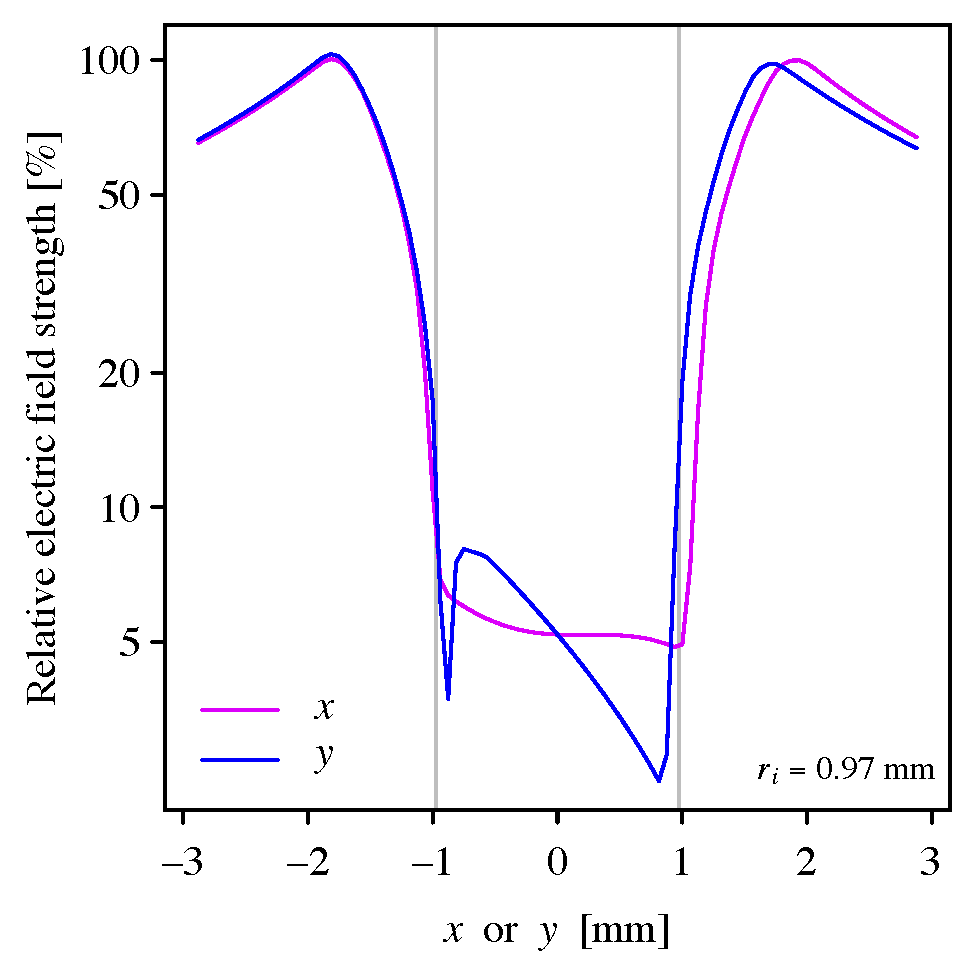
\includegraphics[width=\columnwidth]{CHG1b_170512_8p75A_2-4-2p7kG_500V_76mA_hires_Eslice}
  \caption{Calculated relative electric field for the hollow electron
    gun CHG1b in the transverse $x$-$y$ plane (left) and as
    1-dimensional cuts through the $x$ and $y$ axes (right). The field
    calculations are based on measurements at the Fermilab
    electron-lens test stand combined with Warp calculations of the
    electric potentials and fields in a cylindrical beam pipe.}
\label{core:fig:1}
\end{figure*}

Parasitic kicks on the proton beam core can be due to electron-beam
profile imperfections in the overlap region, or to the injection and
extraction toroidal bends, where electrons and protons overlap, as
shown in the layout of Fig.~\ref{fig:hel_layout}.

Because no HEL is currently installed in the LHC, the kicks on the
proton beam core must be emulated by other devices to determine their
effects experimentally in a given machine and to guide design and
tolerances. In particular, during the experiments presented in this
paper, the LHC transverse damper system (described in detail in
Section~\ref{sec:adt}) was used for this purpose. This system can
generate transverse dipole kicks with a wide range of excitation
patterns.

For comparison with experiments and simulations, here we estimate to
first order the magnitude of the dipole kicks that may be expected
from the HEL. As one can see below, the contribution from the central
region is in general dominating.


\subsection{Kicks from injection and extraction bends}
\label{core:sec:1}

To estimate the dipole component of the kicks that originate from the
injection and extraction bends, we used the approach described in
Ref.~\cite{hel_bends_stancari}. The bends are modeled as a bent
cylindrical pipe with a static charge distribution of electrons. The
resulting electric field is calculated, with the vacuum pipe as
boundary, using the solvers of the Warp particle-in-cell
code~\cite{warp}. (The contribution of the magnetic field generated by
the electron current was neglected in this study.) The field,
integrated over the trajectory of the protons, is then translated into
a symplectic kick map.

In case of a U-shaped electron lens, where electron gun and collector
are on the same side, the transverse (and possibly pulsed) dipole
kicks generated by the electron charge at the entrance and exit add
up. For an S-shaped electron lens, on the other hand, where gun and
collector are on opposite sides, these kicks compensate each
other. For this reason, an S-shape was chosen for the HL-LHC HEL
(Fig.~\ref{fig:hel_layout}). A disadvantage of the S-shape is that the
static magnetic kicks due to the toroidal sections do add up, but they
can be compensated by conventional dipole correctors, especially in a
high-energy machine.

In the case under study of an S-shaped electron lens, residual
uncompensated kicks arise from differences in electron charge
distribution between the injection and extraction bends. Here we
conservatively assume 10\% fluctuations between the entrance and exit
and, furthermore, that these differences add up.

The maximum values of the integrated electric fields calculated in
Ref.~\cite{hel_bends_stancari}, based upon an electron beam of 1~A at
5~keV, are
%
\begin{equation}
  \int_{z_1}^{z_2} E_{x,y} \, dz= \q{10}{kV}.
\end{equation}
%
Scaling to HL-LHC and HEL design parameters
(Table~\ref{tab:hllhc_param} and Table~\ref{tab:hel_param}) yields the
following integrated field and corresponding kick:
%
\begin{equation}
  \int_{z_1}^{z_2} E_{y} \, dz = \q{36}{kV} \Rightarrow \Delta y' = \q{5.1}{nrad},
\end{equation}
%
as described in detail in
Ref.~\cite{md_sim_hel_res_ex_fitterer}. Assuming a residual difference
of 10\% between entrance and exit, the expected kick is approximately
%
\begin{equation}
  \label{eqn:kick_bends}
  \Delta x', \Delta y' = \q{0.5}{nrad}.
\end{equation}


\subsection{Kicks in the central overlap region}
\label{core:sec:2}

For a perfectly annular and axially symmetric electron beam profile,
the electromagnetic field in the region of the proton beam core
vanishes. This is expressed by Eq.~\ref{eq:field_2} and is illustrated
in Fig.~\ref{fig:hel_field}. Fields at the location of the proton beam
core can arise if the axial symmetry is broken.

Recently, a hollow electron gun prototype for the LHC (called CHG1b)
was characterized at the Fermilab electron lens test
stand~\cite{hel_test_stand_fnal}. An example of a measurement of the
electron beam current density is shown in Fig.~\ref{core:fig:0}.

In the test stand, only resistive solenoids are available. One can
estimate the fields generated by the compressed electron beam profile
in the superconducting solenoids of the HL-LHC HEL using a combination
of experimental measurements and calculations.

Experimentally, it was verified that the current-density profiles
scale with electron beam current and confining axial field according
to space-charge evolution~\cite{Jo:PoP:2018,
  hel_res_field_stancari_2017}. Specifically, the same profile is
obtained for a given family of experimental conditions with constant
ratio $\sqrt{V} / B$, where $V$ is the accelerating voltage and $B$ is
the axial field. This ratio is proportional to the space-charge
evolution number $g = \omega_D \cdot \tau \propto \sqrt{V}/B$,
representing the number of $\vec{E} \times \vec{B}$ rotations in the
propagation time~$\tau$, with
$\omega_D \equiv \omega_p^2 / (2 \omega_c)$ the diocotron frequency,
$\omega_p$ the plasma frequency, and $\omega_c$ the cyclotron
frequency of the magnetically confined electrons in the
solenoid~\cite{Davidson:nonneutral-plasmas:2001}.

For a given HL-LHC HEL configuration, the corresponding
current-density profile measured in the Fermilab test stand is used as
input to calculate the electromagnetic fields. For the purpose of
estimating the residual fields, the measured distribution is
compressed to the inner electron beam radius of 1.24~mm, corresponding
to $4\sigma_p$, as described in Table~\ref{tab:hllhc_param} and
Table~\ref{tab:hel_param}. A distribution with about $65\,000$
particles is generated according to the measured current-density
profile. As boundary condition, the LHC inner beam pipe radius
$b = \q{30}{mm}$ is used. The potential and fields are then calculated
with Warp~\cite{warp}. The resulting relative electric field strengths
are shown in Fig.~\ref{core:fig:1}. The electric field is obviously
proportional to the charge density of electrons. Its relative strength
is rather insensitive to the hollow beam radii, as long as these
remain small compared to the beam pipe radius. Further details on the
measurements and Warp simulations can be found in
Ref.~\cite{hel_res_field_stancari_2017}.

Using these measurements and calculations of the relative electric
field strengths in the transverse plane (Fig.~\ref{core:fig:1}), we
obtain a median field in the hole of
%
\begin{equation}
  \langle E_\mathrm{hole} \rangle / E_\mathrm{max} =  5\%.
\end{equation}
%
For a maximum kick of 392~nrad, as derived in Eq.~\ref{eqn:helkick},
the estimated dipole kick amplitude at the proton beam core is therefore
approximately
%
\begin{equation}
  \label{eqn:kick_central}
  \Delta x' , \Delta y' = \q{20}{nrad}.
\end{equation}
%
The relative magnitude of the residual field depends on several
factors, including cathode quality, electron gun geometry, solenoid
field configuration, space-charge evolution, etc. It can be improved,
if needed.

For the purposes of this paper, only the approximate magnitude of the
residual dipole kick is considered. In general, the field map,
including its multipolar components, can be parameterized in
symplectic form, as described for instance in
Ref.~\cite{hel_bends_stancari}, and used in tracking codes to estimate
the effects on the circulating beam.



\section{Experimental setup}
\label{sec:exp}

\begin{table*}
  \caption{Beam parameters and machine configuration for the two
    resonant excitation experiments of~2016
    and~2017~\cite{resexmd2016, resexmd2017}. The plane of the
    excitation is abbreviated as H for horizontal, V for vertical and
    H+V for horizontal and vertical at the same time.}
  \label{tab:md_param}
  \begin{ruledtabular}
    \begin{tabular}{lcc}
      Parameter & Experiment 2016 & Experiment 2017  \\
      \colrule
      beam &\multicolumn{2}{c}{Beam~1} \\
      beam energy &\multicolumn{2}{c}{injection energy, 450 GeV} \\\hline
      single bunch intensity &\multicolumn{2}{c}{$0.7\times10^{11}$} \\
      normalized emittance &\multicolumn{2}{c}{$2.5$--\q{3.5}{\mu m}} \\
      $4\sigma$ bunch length & \multicolumn{2}{c}{1.3~ns}\\
      $1\sigma$ bunch length & \multicolumn{2}{c}{9.7~cm}\\
      number of bunches & $12 \times 4 = 48$ & $3 \times 72 = 216$ \\
                &  & (+ 1 pilot + 12 nominal) \\\hline
      injection optics, $\beta^* = \q{11}{m}$ & standard optics 2016 & standard optics 2017\\
      Landau-damping octupoles  & \multicolumn{2}{c}{$I_{\mathrm{MO}}
                                  = \q{+19.6}{A}$ for MOF circuit and}\\
                & \multicolumn{2}{c}{$I_{\mathrm{MO}} = \q{-19.6}{A}$
                  for MOD circuit (standard 2016 settings)} \\ \hline
      working point $(Q_x, Q_y)$ & (64.28, 59.31) & (62.27, 60.295) \\
      chromaticity $(Q'_x, Q'_y)$ & \multicolumn{2}{c}{(+15, +15)}\\ \hline
      pulsing patterns  & $7^{\mathrm{th}}$~turn H
                                  &$7^{\mathrm{th}}$~turn H, V, H+V \\
                & $10^{\mathrm{th}}$~turn V & $8^{\mathrm{th}}$~turn
                                              H, V, H+V \\
                & &  random  H, V, H+V\\
    \end{tabular}
  \end{ruledtabular}
\end{table*}

\begin{figure*}
  \begin{tabular}{c}
    \multicolumn{1}{l}{\emph{2016 experiment}} \\
    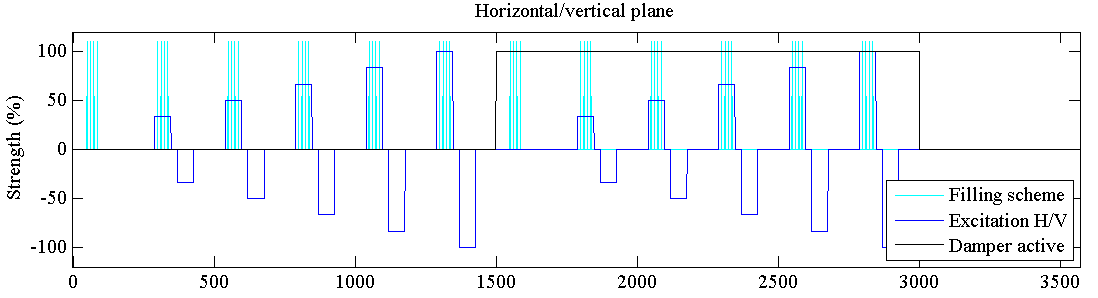
\includegraphics[width=0.95\textwidth]{bunchfilling_2016.png} \\
    \\
    \multicolumn{1}{l}{\emph{2017 experiment}} \\
    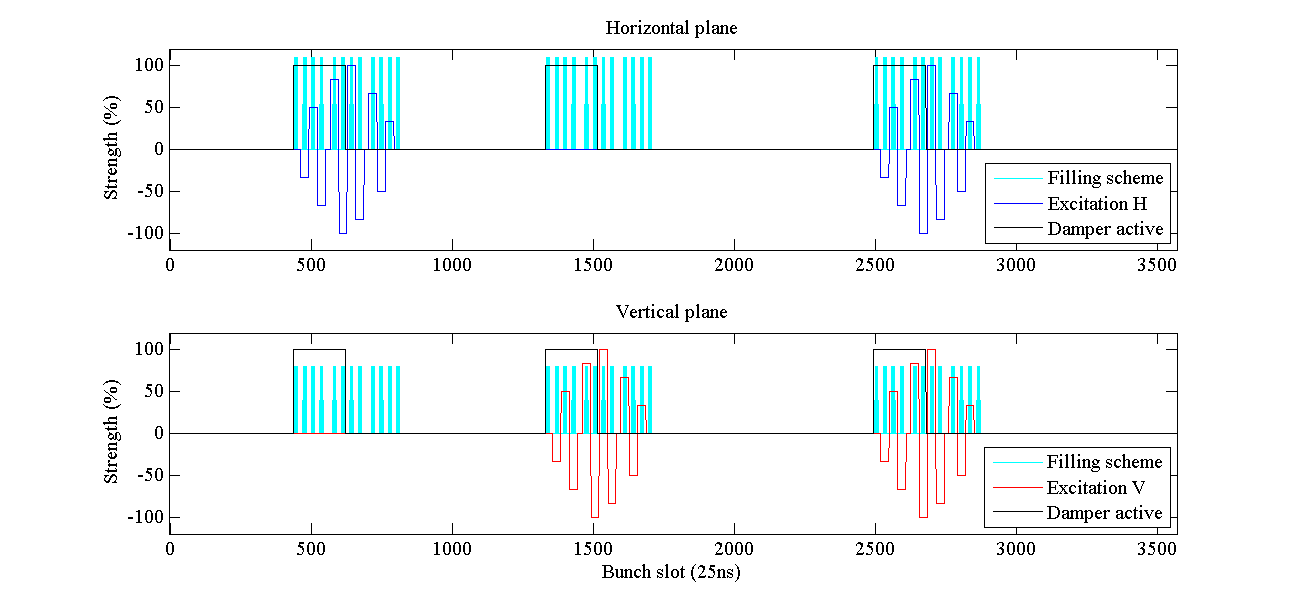
\includegraphics[width=0.95\textwidth]{bunchfilling_2017.png}
  \end{tabular}
  \caption{Bunch filling scheme and excitation patterns for the
    2016~(top) and 2017~(bottom) LHC experiments. In 2016, a total of
    48~bunches was used, whereas in 2017 there were 216~bunches. Each
    bunch is represented by a vertical cyan bar. The bunches were
    grouped in subsets of~4 in 2016 and in subsets of~6 in 2017. Each
    subset experienced the same excitation pattern and amplitude. The
    excitation amplitudes and relative phases are shown in blue or
    red. In 2016, the excitation was only applied in one plane. In
    2017, more injected bunches were allowed without compromising
    machine protection, so it was possible to test all~3 excitation
    planes in the same fill. The transverse damper was active on half
    of the bunches, indicated by the black lines.}
  \label{fig:fill}
\end{figure*}

\begin{figure*}
  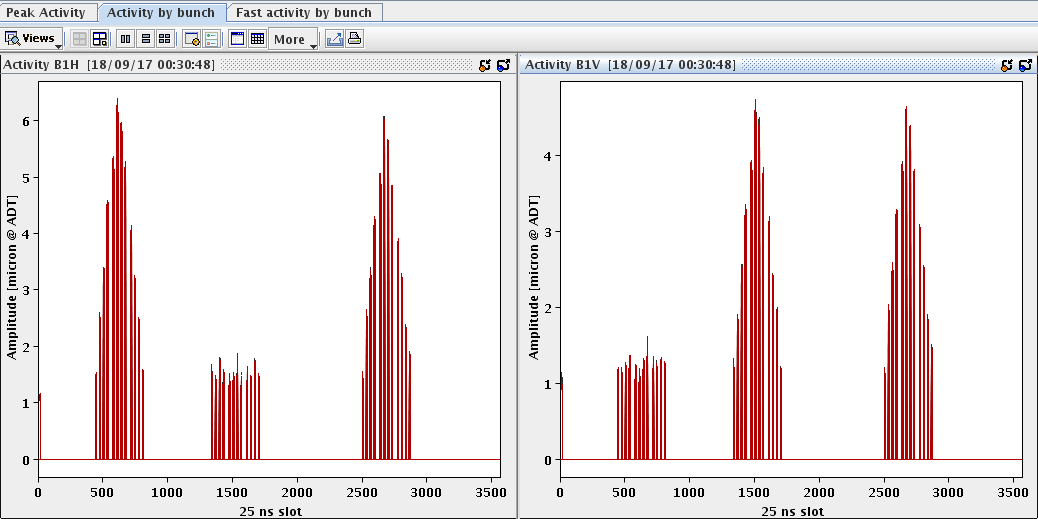
\includegraphics[width=\textwidth]{bunchfilling_measured.png}	
  \caption{Example of bunch-by-bunch beam centroid motion for Beam~1
    in the horizontal (B1H, left) and vertical (B1V, right) planes,
    detected by the real-time transverse activity monitor during the
    2017 experiment, when the beam was excited every
    $8^\mathrm{th}$~turn.}
  \label{fig:fill_meas} 
\end{figure*}

\subsection{Overview}
\label{sec:exp_sum}

The purpose of the experiments at the LHC is to quantify the effects
of a pulsed excitation on the proton beam core. In addition, these
measurements provide an experimental basis to guide the design and
tolerances on the residual HEL fields at the location of the beam
core, in case resonant excitation is needed for HL-LHC.

Two experiments were conducted, one in 2016~\cite{resexmd2016} and one
in 2017~\cite{resexmd2017}. Beam and machine parameters are summarized
in Table~\ref{tab:md_param}.

During the experiments, losses were measured with the fast beam
current transformers (FBCTs). Transverse beam profiles and emittances
were provided by the beam synchrotron radiation telescope (BSRT). All
instruments were capable of delivering bunch-by-bunch data. The data
analysis of the BSRT profiles is quite involved. In this paper, we
focus on the direct comparison of the resulting profiles. A detailed
description of the profile analysis can be found in
Ref.~\cite{bsrtprofinj}, with individual experiments reported in
Refs.~\cite{resexmd2016, resexmd2017}.

The choice of excitation patterns for the experiments was guided by
losses and emittance growths calculated in numerical tracking
simulations, described below. It was chosen to study experimentally
the two pulsing patterns with the largest calculated effects on the
beam ($7^{\mathrm{th}}$- and $10^{\mathrm{th}}$-turn pulsing), one
pattern with no effect ($8^{\mathrm{th}}$-turn pulsing), and the
random excitation. In order to quantify the reproducibility of the
results under different machine configurations, one pulsing pattern
($7^{\mathrm{th}}$-turn pulsing) was tried first in~2016 and then
repeated in~2017.


\subsection{Excitations with the transverse damper and bunch filling schemes}
\label{sec:adt}

The primary function of the LHC transverse damping and feedback
system, also known as ADT, is to mitigate injection oscillations and
to actively damp the coupled-bunch instabilities driven by machine
impedance~\cite{adt_sum_2008, adt_sum_2011}. The main building blocks
of the system are the following: strip-line pickups at positions Q7
and Q9 near Interaction Point~4 (IP4) of the LHC, which are connected
to the beam position measurement modules at the surface; the digital
signal processing modules (mDSPU); and a set of tetrode power
amplifiers feeding electrostatic kickers in the same radio-frequency
sector of the LHC (IP4).

Because of its flexibility and state-of-the-art hardware, the system
is being routinely used for sophisticated beam excitations. These
include abort- and injection-gap cleaning, excitation of individual
bunches for tune and linear-coupling measurements, and other special
modes of operation for dedicated experiments in the LHC.

The transverse feedback is in general active during all phases of LHC
operation. The typical machine cycle requires a short damping time of
10--20 turns (high feedback gain) for injection oscillation
damping. During the acceleration ramp and during collisions, the
damping time is increased to 50--100 turns (lower feedback gain).

Because the damper is always active in operations, it is critical that
the noise introduced by the system does not cause any measurable
emittance growth, and this fact was verified
experimentally~\cite{adt_noise_emit_2017}. All excitation signals
described in this paper were digitally synthesized in the ADT's
digital signal processing units and are therefore assumed to be
`noise-free.' The observed effects on the beam are attributed to the
applied excitations and the effects of unwanted residual noise are
assumed to be negligible.

The resonant excitation experiment in~2017 involved simultaneous
measurements on 3~groups of 72~bunches, with dedicated excitation
patterns and transverse feedback configurations (i.e., damper active
or damper off) on each subset of 6~bunches. In~2016, a similar
configuration was used, with 48~bunches in total and subsets of
4~bunches. Both schemes are illustrated in Fig.~\ref{fig:fill}. A
total of 5 different amplitudes could be applied simultaneously to
different subsets of bunches, denoted as $n \, \Delta A$, with
$n = 1, \ldots, 5$. In addition, there were reference bunches without
excitation for each transverse feedback configuration and excitation
plane. Observables (losses, emittances, etc.) were averaged over each
subset of bunches experiencing the same excitation and damping
conditions.

In~2017, the excitations in the horizontal and vertical planes were
generated by a different set of signal-processing devices, but
synchronized at a turn-by-turn level. Therefore, the bunches of the
third group of 72 bunches (see Fig.~\ref{fig:fill}) were affected by
the kicks in both horizontal and vertical planes during the same turn.

The experiments were usually split in time into 3 different periods:
%
\begin{description}
\item[Period 1] No excitation was applied, to allow the beam to reach
  an equilibrium state after injection.
\item[Period 2] The excitation was applied with a first maximum
  excitation amplitude of $A_{\mathrm{max,1}} = 5 \, \Delta A_1$.
\item[Period 3] The maximum excitation amplitude was further increased
  to $A_{\mathrm{max,2}} = 5 \, \Delta A_2 > A_{\mathrm{max,1}}$.
\end{description}
%
Each period lasted approximately 10--15~minutes, which was considered
long enough to allow the beam to reach its new equilibrium state. In
the discussion of the experimental results (Section~\ref{sec:simex}
below), the 3~periods are labeled according to the maximum excitation
amplitude~$A_\mathrm{max}$, and subsets of bunches with the same
excitation amplitude $n \, \Delta A$ ($n = 1, \ldots, 5$) are grouped
by color.

The proton deflection angle generated by the ADT kicker was calculated
from the kicker geometry and from the excitation voltage on the
deflection plates. The voltage depends on a complex chain of hardware
(digital signal processor, transmission lines, low- and high-power
amplifiers, etc.). In~2016, the kick was estimated from the
operational system parameters and it was assigned an uncertainty of
50\%. In~2017, the excitation voltage could be indirectly measured
once, using the probes mounted on the kickers, with an estimated
uncertainty of 10--15\%. A precise in-situ calibration was not
possible due to the limited machine availability for dedicated
studies.

The maximum ADT kick strength that could be obtained at injection
without risking saturation was approximately 100~nrad. For the
experiments, a maximum nominal kick strength of 96~nrad was chosen.

Figure~\ref{fig:fill_meas} shows an example of the oscillation
amplitude of each bunch centroid in both horizontal and vertical
planes, captured by the LHC real-time transverse activity monitor
during the 2017 experiments, when the beam was excited every
$8^{\mathrm{th}}$~turn. The measured activity shows the typical
amplitude of bunch centroid excursions and reflects the expected
excitation pattern.



\section{Numerical tracking simulations}
\label{sec:sim}

\begin{table*}
  \caption{Summary of parameters used in numerical simulations of
    distribution tracking and frequency-map analysis (FMA). Further
    details can be found in Refs.~\cite{md_sim_hel_res_ex_fitterer,
      resexmd2017}.}
  \label{tab:sim_param}
  \begin{ruledtabular}
    \begin{tabular}{lcc}
      Parameter & distribution & FMA \\
      \colrule
      beam &\multicolumn{2}{c}{Beam~1} \\
      beam energy &\multicolumn{2}{c}{450 GeV} \\
      normalized emittance & \q{3.5}{\mu m} & \q{2.5}{\mu m} \\
      $4\sigma$ bunch length & \multicolumn{2}{c}{1.3~ns} \\
      $1\sigma$ bunch length & \multicolumn{2}{c}{9.7~cm} \\
      particle distribution & \parbox{0.4\textwidth}{6D Gaussian
                              distribution with $10^4$ particles}
                               & \parbox{0.4\textwidth}{equally spaced
                                 grid in $x, y$ up to $10\sigma$, with
                                 $(\Delta p / p_0) = 0$} \\
      turns tracked & $10^6$ & $10^4$ \\
      \hline
      optics & \multicolumn{2}{c}{2016 or 2017 injection optics, with
               $\beta^* = \q{11}{m}$ at IP1 and IP5} \\
      machine imperfections & standard errors, with $a_1 = b_1 =
                              0$\footnote{Orbit
                              errors are disabled due to
                              different implementation of the
                              $a_1, b_1$ coefficients in Lifetrac and
                              MAD-X. $b_2$ errors are adjusted to
                              yield an average
                              peak $\beta$-beat of 15\% over 60~seeds, as
                              observed in optics measurements
                              in the LHC.} & no errors \\
      octupoles  & \multicolumn{2}{c}{$I_{\mathrm{MOF}} =
                   \q{+19.6}{A}$, $I_{\mathrm{MOD}} = \q{-19.6}{A}$} \\
      tunes $(Q_x, Q_y)$ & \multicolumn{2}{c}{(64.28, 59.31) for 2016,
                           (62.27, 60.295) for 2017} \\
      chromaticities $(Q'_x, Q'_y)$ & \multicolumn{2}{c}{(+15, +15)} \\
      \hline
      transverse aperture & $5.7\sigma$ &  \\
      longitudinal aperture & $10\sigma$ &  \\
    \end{tabular}
  \end{ruledtabular}
\end{table*}

For the preparation and interpretation of the experiments, two
different types of simulations were performed:
%
\begin{itemize}
\item tracking of a Gaussian distribution, referred to as
  `distribution tracking' in this paper, to obtain particle loss rates
  and emittance evolution;
\item frequency-map analysis (FMA), to visualize the location and
  intensity of resonances~\cite{fmalaskar}.
\end{itemize}
%
For both simulation types, the tracking code Lifetrac~\cite{lifetrac}
was used. The simulation parameters are summarized in
Table~\ref{tab:sim_param}. Further details are given in
Refs.~\cite{md_sim_hel_res_ex_fitterer, resexmd2017}.

Quantitative predictions of loss rates and emittance growth are in
general challenging, as both observables are influenced by several
factors. For instance, the natural noise present in the machine
(originating from mechanical vibrations, current ripple in the magnet
power supplies, etc.) may have complex interactions with the external
excitations. In the LHC, noise sources at top energy are well
characterized, whereas they are not well known at injection,
presenting an influential but undefined input for simulations.

Collective effects, such as intra-beam scattering and electron cloud,
influence the time evolution of losses and emittance as well. To
minimize their effects, experiments were done at low bunch intensities
($0.7 \times 10^{11}$ protons per bunch). The presence of collective
effects was neglected in these simulations.

The results of tracking simulations are discussed below in
Section~\ref{sec:simex} together with the experimental results, to
enhance the understanding and interpretation of the models and
observations.



\section{Results}
\label{sec:simex}

In this Section, we present the experimental observations and compare
them with the results of numerical simulations.  In
Section~\ref{sec:pattern}, we show which pulsing patterns are most
efficient in the LHC, using the 2016 experiments as an example to show
that these patterns can be predicted.  Next, we present results for
each of the specific excitation patterns that could be tested
experimentally, namely pulsing every $10^{\mathrm{th}}$~turn
(Section~\ref{sec:simex10}), $7^{\mathrm{th}}$~turn
(Section~\ref{sec:simex7}), $8^{\mathrm{th}}$~turn
(Section~\ref{sec:simex8}), and the random excitation
(Section~\ref{sec:simexran}).  In Section~\ref{sec:damp}, we describe
how the transverse damping system influenced the effects of the
external excitation sources on losses, beam distributions, and
emittances.


\subsection{Dependence on the pulsing pattern\label{sec:pattern}}
The effect of each pulsing pattern in comparison to the other patterns can be identified by the means of the loss rate and emittance growth from the distribution tracking. As an example, the simulation results for the 2016 experiment are shown in Fig.~\ref{fig:patternsim} featuring a clear dependence of both parameters on the pattern.
\begin{figure*}[h]
	\begin{minipage}[t]{0.49\linewidth}
		\centering
		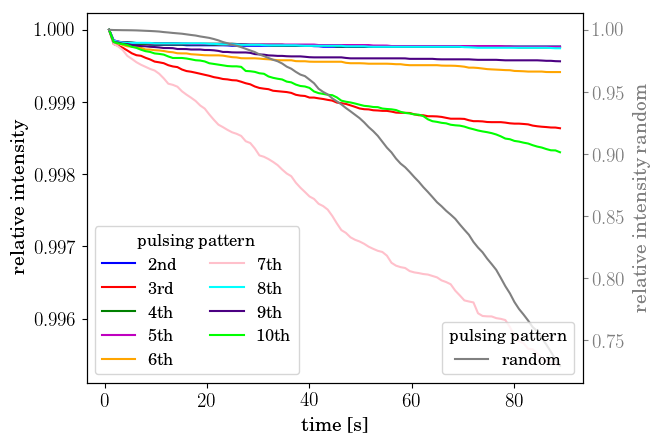
\includegraphics[width=1.0\linewidth]{2016injerra2b2u_pattern_3_5um_intensity.png}
	\end{minipage}
	\begin{minipage}[t]{0.49\linewidth}
		\centering
		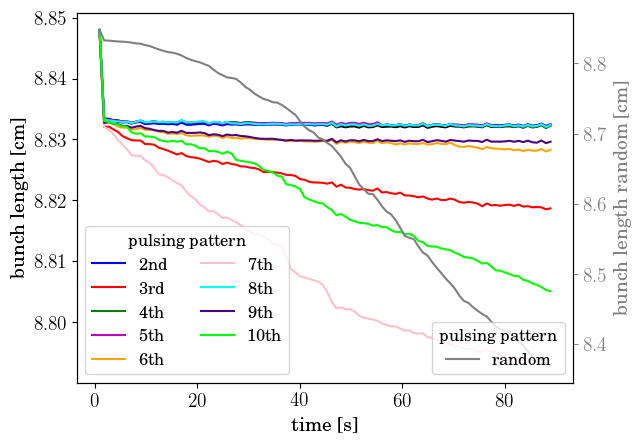
\includegraphics[width=1.0\linewidth]{2016injerra2b2u_pattern_3_5um_sigm.png}
	\end{minipage}	
	\begin{minipage}[t]{0.49\linewidth}
		\centering
		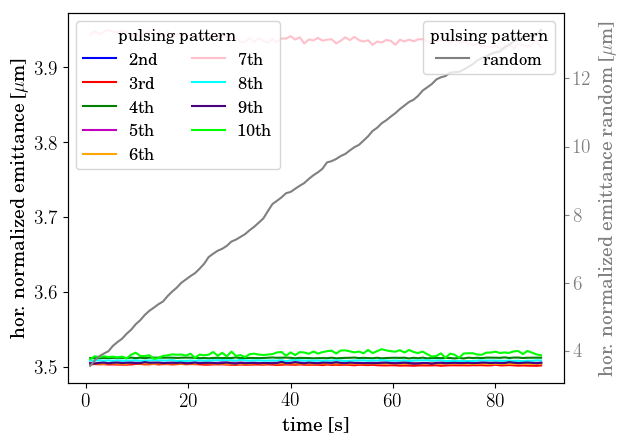
\includegraphics[width=1.0\linewidth]{2016injerra2b2u_pattern_3_5um_emit1.png}
	\end{minipage}
	\begin{minipage}[t]{0.49\linewidth}
		\centering
		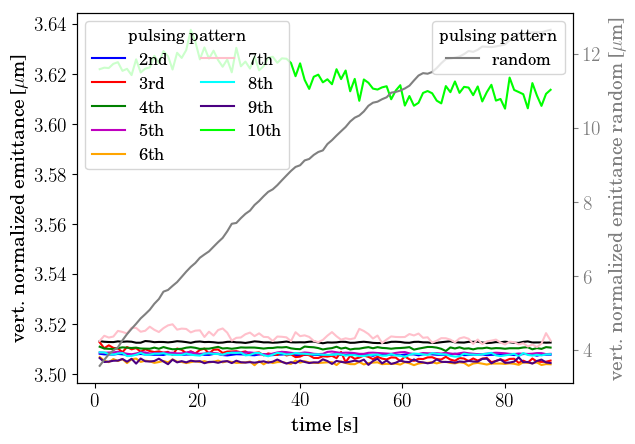
\includegraphics[width=1.0\linewidth]{2016injerra2b2u_pattern_3_5um_emit2.png}
	\end{minipage}	
	\caption{\label{fig:patternsim} Relative intensity (top left), bunch length (top right) and horizontal (bottom left) and vertical (bottom right) emittance for different pulsing patterns obtained from distribution tracking based on the 2016 injection optics with $(Q_x,Q_y)=(64.28,59.31)$ with standard errors. The resonant and random excitation respectively is applied in both planes with an amplitude of 96~nrad. No random noise component is added in addition.}
\end{figure*}

The largest losses are observed for $3^{\mathrm{rd}}$, $7^{\mathrm{th}}$ and $10^{\mathrm{th}}$~turn pulsing and a uniform random excitation. As the bunch length decreases in accordance with the losses, the losses can be mostly associated to off-momentum particles hitting the transverse aperture. Only $7^{\mathrm{th}}$ and $10^{\mathrm{th}}$~turn pulsing as well as random excitation exhibit considerable emittance growth. Compared to any resonant excitation, the random excitation has by far the strongest effect.

The sensitivity to $7^{\mathrm{th}}$ and $10^{\mathrm{th}}$~turn pulsing is also observed in absence of machine errors in which case the only source of non-linearities are sextupoles and octupoles~\cite{md_sim_hel_res_ex_fitterer} suggesting that latter are responsible for the observed sensitivity. The driven resonances are revealed by the FMA analysis shown in Fig.~\ref{fig:patternfma}. The $7Q_x$ resonance is excited in case of the $7^{\mathrm{th}}$~turn pulsing and the $10Q_x$ and $10Q_y$ resonance in case of the $10^{\mathrm{th}}$~turn pulsing. As octupoles can only drive even resonances, the source of the $7Q_x$ resonances are the sextupoles while the octupoles only generate the tune footprint. The other pulsing patterns do not exhibit any increase in losses or emittance growth without magnetic errors and their effect can be thus attributed to the magnetic field errors, implying also the seed chosen for the simulation.
\begin{figure*}[h]
	\begin{minipage}[t]{0.49\linewidth}
		\centering
		no excitation
		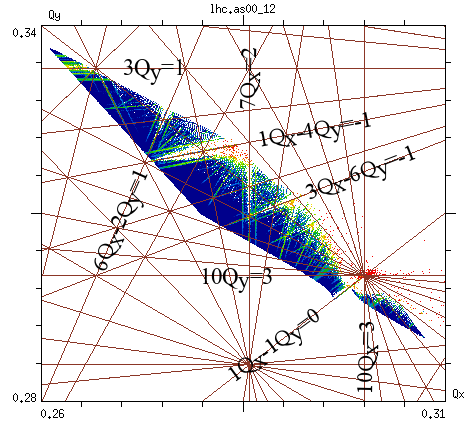
\includegraphics[width=1.0\linewidth]{2016injnocolc15o+19_6noerru_dp0_ord10_annotate.png}
	\end{minipage}
	\begin{minipage}[t]{0.49\linewidth}
		\centering
		$10^{\mathrm{th}}$ H+V
		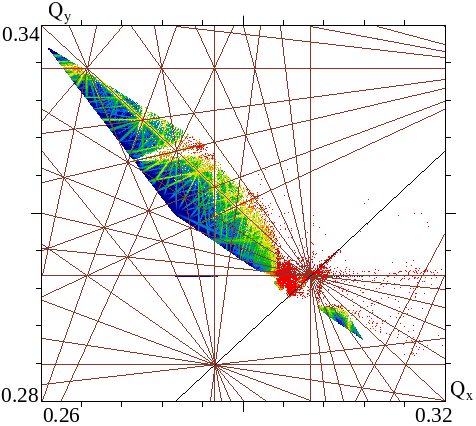
\includegraphics[width=1.0\linewidth]{2016injnocolc15o+19_6noerrut10skhv_dp0_ord10.png}
	\end{minipage}	
	\begin{minipage}[t]{0.49\linewidth}
		\centering
		$7^{\mathrm{th}}$ H
		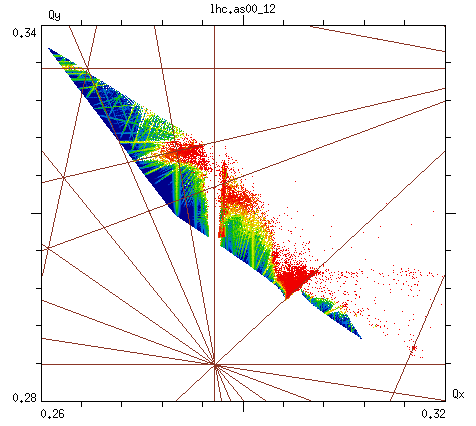
\includegraphics[width=1.0\linewidth]{2016injnocolc15o+19_6noerrut7skh_dp0_ord7.png}
	\end{minipage}	
	\begin{minipage}[t]{0.49\linewidth}
		\centering
		$7^{\mathrm{th}}$ V
		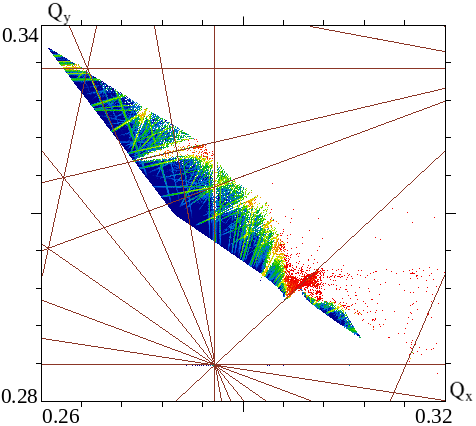
\includegraphics[width=1.0\linewidth]{2016injnocolc15o+19_6noerrut7skv_dp0_ord7.png}
	\end{minipage}
	\caption{\label{fig:patternfma} FMA analysis without excitation (top left) for $10^{\mathrm{th}}$~turn pulsing in H+V (top left) and for $7^{\mathrm{th}}$~pulsing only in H (bottom left) and only in V (bottom right) and  based on the 2016 injection optics with no machine errors and a tune of (64.28,59.31). The excitation is 120~nrad in the corresponding plane. The absence of a strong excitation of any resonance in case of $7^{\mathrm{th}}$~turn pulsing only in V and the strong excitation in case of pulsing only in H confirms the excitation of the $7Q_x$ resonance. For $10^{\mathrm{th}}$~turn pulsing there is in contrast no significant difference between pulsing only in H, only in V or in H+V (see Appendix~\ref{app:sec:10}, Fig.~\ref{app:fig:fma:10}).}
\end{figure*}  

One may have noticed that the emittance in case of the $7^{\mathrm{th}}$ and $10^{\mathrm{th}}$~turn pulsing starts at an increased initial value and then stays almost constant during the entire simulation time, which usually points to an error in the chosen simulation setup. This behavior is however typical for any resonant excitation and can be ascribed to the adjustment of the beam distribution during the first $10^4$ turns to a new equilibrium. As the beam distribution is only dumped every $10^4$ turns, this initial fast adjustment manifests itself in an increased initial emittance value in Fig.~\ref{fig:patternsim}, and also any other simulations over $10^6$ turns presented in this paper. Besides an increased emittance, the new distribution also becomes non-Gaussian. This is illustrated by means of the residual in respect to the Gaussian distribution for $7^{\mathrm{th}}$ and $10^{\mathrm{th}}$~turn pulsing in Fig.~\ref{fig:patternhist}. This initial fast change of the beam distribution is not an artifact of the simulation, but has been, to the knowledge of the authors, also for the first time experimentally observed during the 2016 and 2017 LHC experiments presented in this paper. The timescale of this fast adjustment is in experiments however much slower than predicted in simulations --- on the timescale of minutes compared to seconds. 
\begin{figure*}[t]
	\begin{minipage}[t]{0.49\linewidth}
		\centering
		$7^{\mathrm{th}}$ H+V
		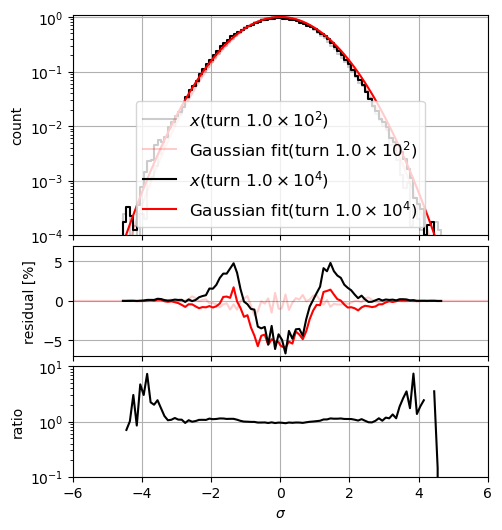
\includegraphics[width=1.0\linewidth]{2016injerra2b2u_t7skhv_3_5um_hist_x.png}
	\end{minipage}
	\begin{minipage}[t]{0.49\linewidth}
		\centering
		$10^{\mathrm{th}}$ H+V
		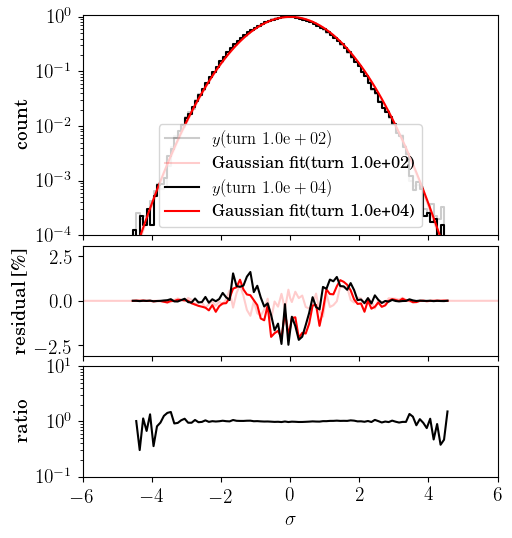
\includegraphics[width=1.0\linewidth]{2016injerra2b2u_t10skhv_3_5um_hist_y.png}
	\end{minipage}	
	\begin{minipage}[t]{0.49\linewidth}
		\centering
		random H+V
		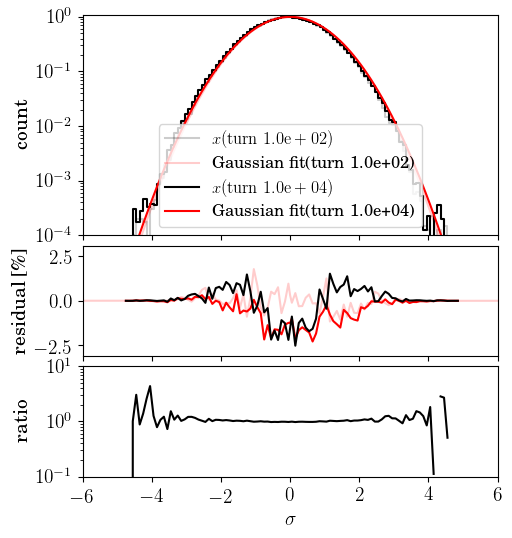
\includegraphics[width=1.0\linewidth]{2016injerra2b2u_ranhv_3_5um_hist_x.png}
	\end{minipage}
	\begin{minipage}[t]{0.49\linewidth}
		\centering
		no excitation
		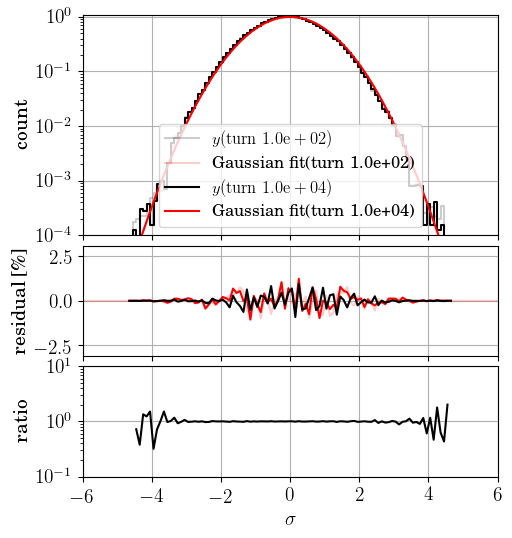
\includegraphics[width=1.0\linewidth]{2016injerra2b2u_3_5um_hist_y.png}
	\end{minipage}	
	\caption{\label{fig:patternhist} Horizontal beam distribution for $7^{\mathrm{th}}$~turn pulsing (top left), vertical beam distribution for $10^{\mathrm{th}}$~turn pulsing (top right) and horizontal (bottom left) and vertical (bottom right) beam distribution for random excitation from distribution tracking simulations based on the 2016 injection optics with $(Q_x,Q_y)=(64.28,59.31)$ and standard errors. The excitation is applied in both planes with an amplitude of 96~nrad. The residual is defined as the final distribution (here after $10^4$~turns) minus the initial distribution (here after $10^2$~turns) as \%, and the ratio as the final distribution divided by the initial distribution. The red line in the plot of the residual is the difference between the Gaussian fit of the distribution and the distribution itself.}
\end{figure*}

In the presence of only a resonant excitation, this modified distribution is stable in simulations with a constant emittance. As we will see later, an increase of the emittance with the applied excitation amplitude is however observed experimentally not matching the prediction by simulations. By adding a random noise component representative for the natural noise present in the LHC, the constant emittance is changed in simulations to an excitation amplitude dependent emittance growth after an initial adjustment phase. In case of random uniform noise, the excitation leads to constant emittance growth without any initial adjustment phase. The interaction with the natural noise source then only results in an underestimation of loss rates and emittance growth as it is basically equivalent to the application of random noise with an increased amplitude. In addition to the experiments presented in this paper, the effect of a random excitation was also studied in a separate experiment at the LHC for the case of colliding beams \cite{md1433_noise_top_energy,md_noise_bbLHC}.

\clearpage

\subsection{$10^{\mathrm{th}}$ turn pulsing\label{sec:simex10}}
The $10^{\mathrm{th}}$~turn pulsing pattern was tested in 2016 with an excitation in the vertical plane only. As this was the first time a resonant excitation was tested in the LHC, only in total 48~bunches could be injected in order to still guarantee the protection of the machine. To test different excitation amplitudes during one fill and have enough statistics, the excitation was therefore only applied in one plane. As described earlier, the experiment started with a period of 12~minutes without excitation in order to let the beam distribution fully adjust to its equilibrium state after injection. Afterwards the excitation was applied with the excitation scheme shown in Fig.~\ref{fig:fill} and a maximum excitation amplitude of $A_{\mathrm{max}}=5\Delta A = 48~$nrad for a total of 11~minutes. The excitation was then further increased to the maximum value reachable without saturation of $A_{\mathrm{max}}=5\Delta A = 96~$nrad and kept for 11~minutes. In both cases, the excitation induced the following changes:
\begin{enumerate}
	\item Increase of the loss rate with the excitation amplitude (Figs.~\ref{fig:10thexp}.
	\item Increase of the emittance growth with the excitation amplitude in the vertical plane but not in the horizontal plane (Fig.~\ref{fig:10thexp}).
	\item Change of the beam distribution for the excited bunches (Fig.~\ref{fig:10thexpprof}).	
\end{enumerate}
As loss rates, emittance growth and beam distribution stayed unchanged for the $4$~reference bunches, the above observations can be also truly associated with the effect of the $10^{\mathrm{th}}$~turn pulsing.
\begin{figure*}[h]
	\begin{minipage}[t]{0.32\linewidth}
		\centering
		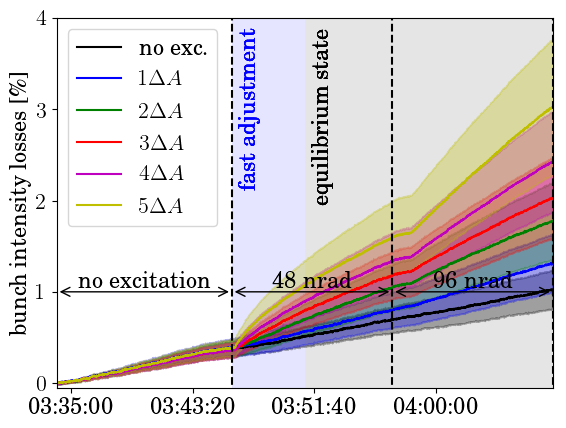
\includegraphics[height=0.75\linewidth]{2016_bunch_intensity_v10th_no_damper_avg.png}
	\end{minipage}
	\begin{minipage}[t]{0.32\linewidth}
		\centering
		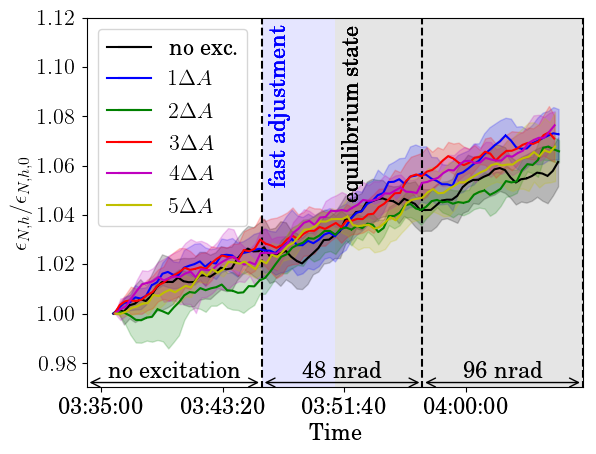
\includegraphics[height=0.75\linewidth]{2016_emith_avg_rel_v10th_no_damper.png}
	\end{minipage}	
	\begin{minipage}[t]{0.32\linewidth}
		\centering
		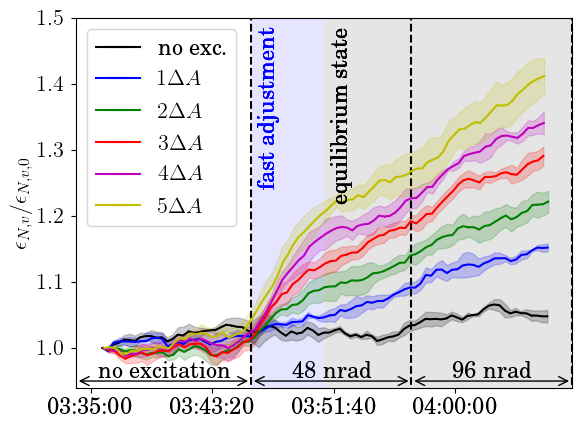
\includegraphics[height=0.75\linewidth]{2016_emitv_avg_rel_v10th_no_damper.png}
	\end{minipage}	
	\caption{\label{fig:10thexp} Relative intensity (top) and relative horizontal (bottom left) and vertical (bottom right) emittance averaged over the bunches experiencing the same excitation amplitude during the 2016 experiments and for $10^{\mathrm{th}}$~turn pulsing in~V. For all bunches the damper was not active. Relative refers here to the normalization to the initial value. For each maximum amplitude $A_{\mathrm{max}}=48$~nrad and 96~nrad indicated with black arrows, the excitation amplitude was linearly increased for each group of 4~bunches (see Fig.~\ref{fig:fill}). The different colored solid lines labeled with $n\Delta A$ are the average over the 4~bunches with the same excitation amplitude together with the $1\sigma$ standard deviation shown as envelope. The area with a blue background indicates the fast adjustment period of the beam distribution transitioning into a new equilibrium state highlighted with a gray background.}
\end{figure*}
These experimentally obtained scalings of the loss rate and emittance growth with the excitation amplitude can be then used for the actual specification of the hollow electron lens.

Besides the numerical determination of tolerances, the vertical emittance actually features indeed the strange and interesting behavior predicted in simulations: a fast adjustment phase of the beam distribution visible as a rapid increase of the emittance followed by the reach of a new equilibrium distribution apparent by a slower continuous emittance growth. These two phases are indicated in Fig.~\ref{fig:10thexp} in blue and black.

\begin{figure*}[h]
	\begin{minipage}[t]{0.49\linewidth}
		\centering
		reference bunch, no excitation
		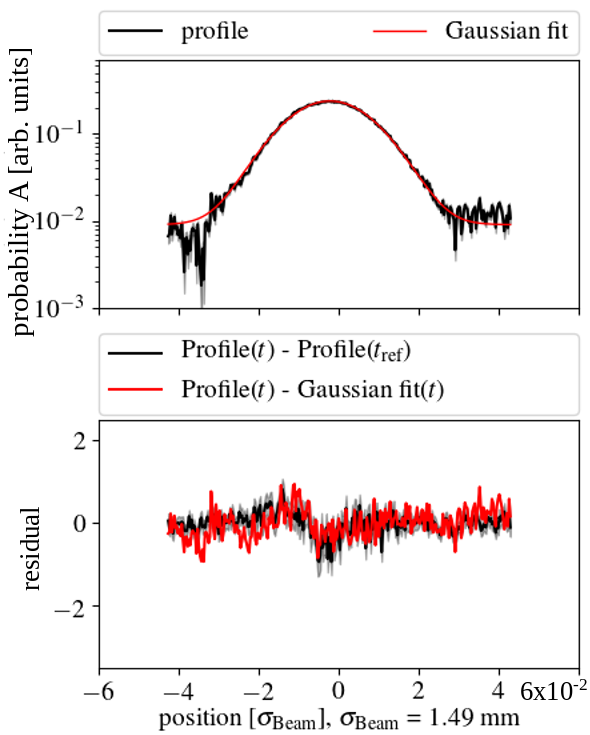
\includegraphics[width=1.0\linewidth]{profile_v_10thv_slot_50.png}
	\end{minipage}
	\begin{minipage}[t]{0.49\linewidth}
		\centering
		excited bunch, $10^{\mathrm{th}}$~turn V		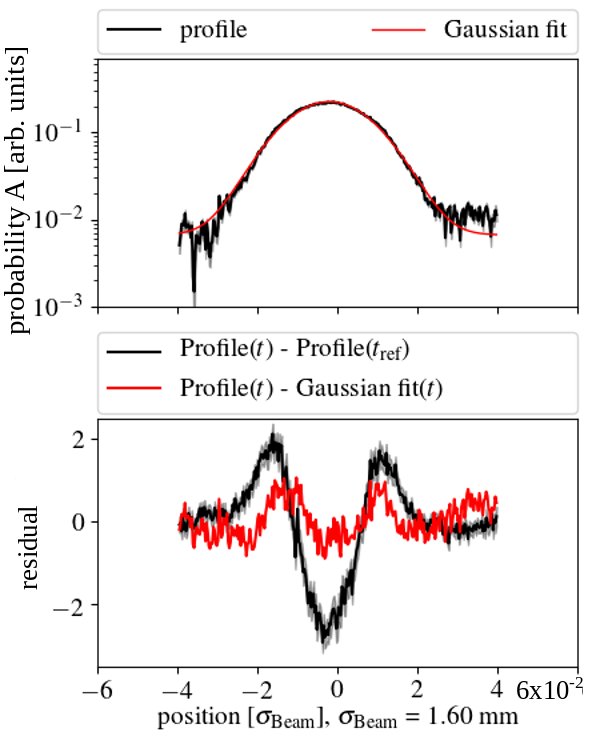
\includegraphics[width=1.0\linewidth]{profile_v_10thv_slot_1300.png}
	\end{minipage}
	\caption{\label{fig:10thexpprof} Vertical beam profiles measured with the Beam Synchrotron Radiation Telescope (BSRT) during the 2016 experiments. The profiles are taken at the end of the $10^{\mathrm{th}}$~turn pulsing in V. For both bunches the transverse damper is not active. The black line in the plot of the residual is the current profile minus the profile before applying the excitation and is a measure for the overall change of the distribution. The red line is the current profile minus its Gaussian fit, which gives and indication for the deviation of the distribution from a Gaussian distribution. For details on the analysis it is referred to \cite{bsrtprofinj}. The distribution of the reference bunch (left), here slot 50, stays unchanged, while the bunch experiencing the maximum excitation (right), here slot 1300, clearly shows a change to a non-Gaussian distribution.}
\end{figure*}
Thanks to the good performance of the Beam Synchrotron Radiation Telescope (BSRT)~\cite{bsrtprofinj}, the distribution changes indirectly observed as changes of the emittance could also be for the first time directly measured. As example Fig.~\ref{fig:10thexpprof} shows the vertical profile of a reference bunch and one bunch experiencing the maximum excitation of $5\cdot\Delta A=A_{\mathrm{max}}=48$~nrad and afterwards 96~nrad. The distribution of the excited bunch not only changes but becomes clearly non-Gaussian, while the reference bunch stays unchanged.
\begin{figure*}[h]
	\begin{minipage}[t]{0.49\linewidth}
		\centering
		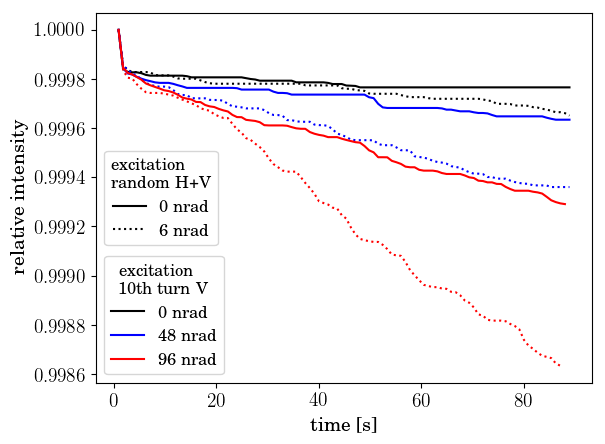
\includegraphics[width=1.0\linewidth]{2016injerra2b2uran1_2e-3_10thV_3_5um_intensity.png}
	\end{minipage}
	\begin{minipage}[t]{0.49\linewidth}
		\centering
		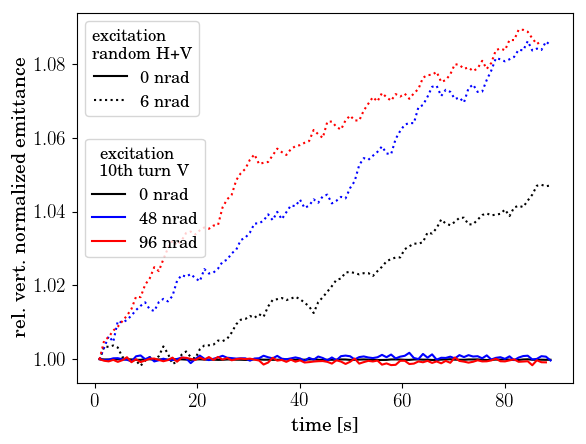
\includegraphics[width=1.0\linewidth]{2016injerra2b2uran1_2e-3_10thV_3_5um_emit2_rel.png}
	\end{minipage}
	\begin{minipage}[t]{0.49\linewidth}
		\centering
		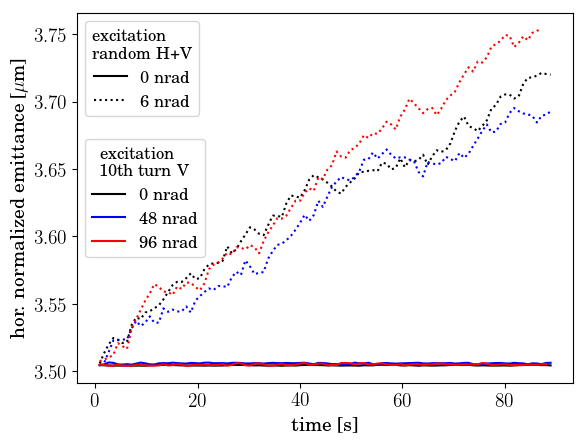
\includegraphics[width=1.0\linewidth]{2016injerra2b2uran1_2e-3_10thV_3_5um_emit1.png}
	\end{minipage}	
	\begin{minipage}[t]{0.49\linewidth}
		\centering
		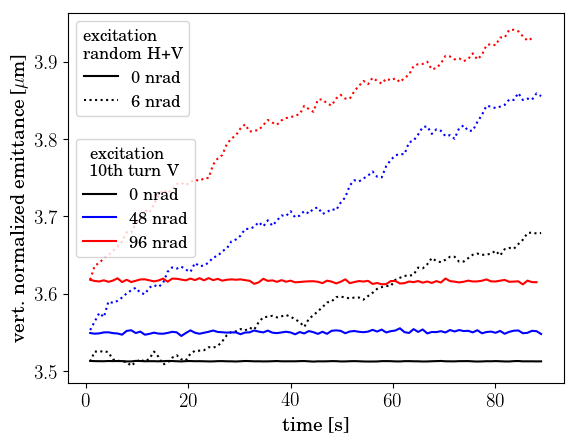
\includegraphics[width=1.0\linewidth]{2016injerra2b2uran1_2e-3_10thV_3_5um_emit2.png}
	\end{minipage}	
	\caption{\label{fig:10thsim} Relative intensity (top left) and relative vert. emittance (top right), and hor. (bottom left) and vert. (bottom right) emittance obtained from simulations (distribution tracking) based on the 2016 injection optics with standard errors and $(Q_x,Q_y)=(64.28,59.31)$. The solid line indicates an excitation with only $10^{\mathrm{th}}$~turn pulsing in V and the dotted line with $10^{\mathrm{th}}$~turn pulsing in V plus a random dipole noise component in H+V of 6~nrad.}
\end{figure*}
The simulation results from the distribution tracking for $10^{\mathrm{th}}$~turn pulsing and without (solid line) and with (dotted line) additional random noise component to emulate the natural noise present in the LHC are shown in Fig.~\ref{fig:10thsim}. As no estimate of the natural noise is available at injection for the LHC, a first estimate is obtained by scaling the estimate for 6.5~TeV \cite{md1433_noise_top_energy,md_noise_bbLHC} by the magnetic rigidity to the injection energy of 450~GeV. This yields a maximum kick amplitude at the transverse damper of approximately
\begin{equation}
\theta_{\mathrm{random,ADT,max}}(\mathrm{450~GeV}) = 6~\mathrm{nrad}.
\end{equation}
As can be seen from simulations, adding a random noise component not only yields the correct qualitative behavior of the emittance but also increases the losses. As the losses are in general underestimated in simulations compared to the experimental results, the discrepancy between simulations and experiment can be thus reduced.  To better compare the experimental results for the two different maximum excitation amplitudes applied for slightly different time intervals and also the simulations conducted for a much shorter interval of only 90~s, we define the relative loss rate $R$:
\begin{equation}\label{eqn:lossrate}
R = \frac{I_{\mathrm{start}}-I_{\mathrm{end}}}{I_{\mathrm{start}}\cdot \Delta t}
\end{equation}
where $I$ is the intensity and $\Delta t$ the time interval during which the excitation with fixed $A_{\mathrm{max}}$ is applied during the experiments or the duration of the simulation respectively. A qualitative comparison of the loss rates obtained in experiments and simulations is shown in Fig.~\ref{fig:10thexploss} featuring a surprisingly good agreement. It should be also kept in mind that the additional random noise component considerably influences the simulation results and as long as it is unknown should be seen more as a fit parameter than a real experimentally confirmed input parameter. The measured loss rates for $A_{\mathrm{max}}=48$~nrad and $A_{\mathrm{max}}=96$~nrad should furthermore follow the same scaling. Instead the loss rates for the same excitation amplitude are smaller for $A_{\mathrm{max}}=96$~nrad compared to $A_{\mathrm{max}}=48$~nrad. That losses and also emittance growth for a fixed excitation amplitude do not exactly agree for both experiments, is a general tendency observed in all experiments. As the second excitation however starts from an already by the previous excitation changed beam distribution, the difference is however not surprising and can be explained by this difference in initial conditions. For checking the reproducibility of the results in a possible future experiment, it would be interesting to see if the same loss rates are measured if for each $A_{\mathrm{max}}$ a new fill is used. 
\begin{figure}[h]
		\centering
%		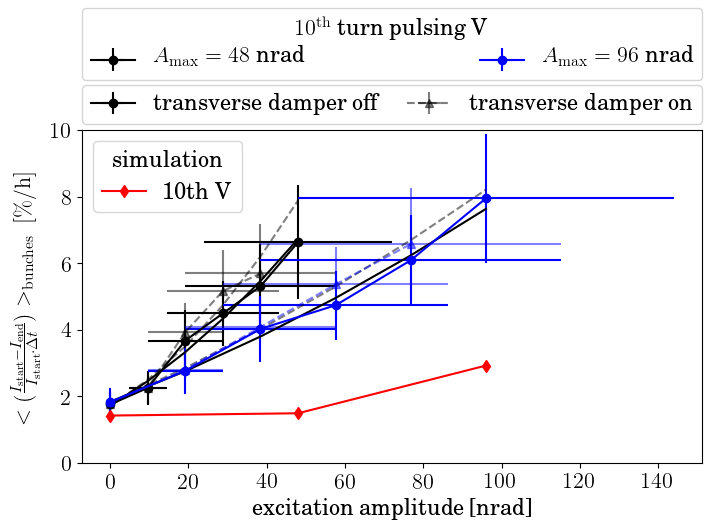
\includegraphics[width=0.8\linewidth]{2016_scale_amp_10v_ran_lbllong_sim.png}
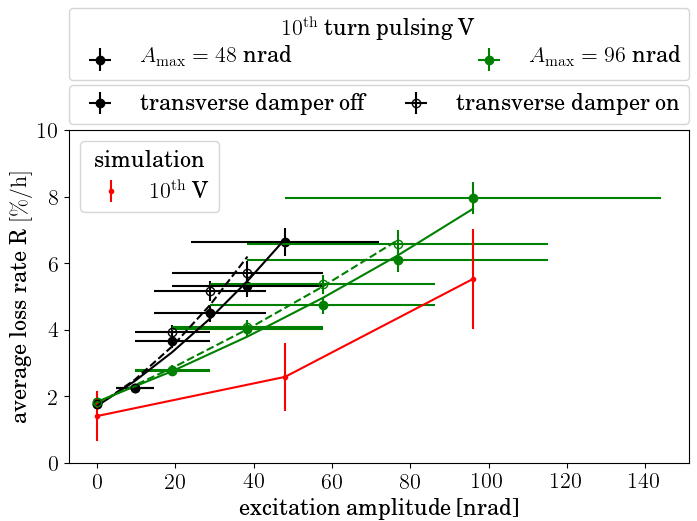
\includegraphics[width=1.0\linewidth]{2016_scale_amp_10v_ran_lblshort_sim_prstab.png}
	\caption{\label{fig:10thexploss} Comparison of scaling of loss rates $R$ as defined in Eqn.~\ref{eqn:lossrate} with the excitation amplitude for $10^{\mathrm{th}}$~turn pulsing in~V. The experimental results for a maximum excitation of $A_{\mathrm{max}}=48$~nrad are shown in black and for $A_{\mathrm{max}}=96$~nrad in green. The excitation amplitude error is 50\% and the error on the loss rate is the pure statistical error on the mean. The simulation results (see Fig.~\ref{fig:10thsim}) for 2016 injection optics, standard errors, $(Q_x,Q_y)=(64.28,59.31)$, $10^{\mathrm{th}}$~turn pulsing in V plus random dipole noise in H+V of 6~nrad are shown in red together with their statistical error. The loss rates follow approximately a quadratic behavior illustrated by a second order polynomial fit to the data shown as solid (for bunches with transverse damper off) or dashed (for bunches with transverse damper on) line.}
\end{figure}

\clearpage

\subsection{$7^{\mathrm{th}}$ turn pulsing\label{sec:simex7}}
The $7^{\mathrm{th}}$~turn pulsing pattern has been tested during both experiments in 2016 and 2017. In 2016 the resonant excitation was tested for the first time in the LHC and the experiments were therefore still in the exploratory state. Based on the experience gained in 2016, the experiments could then be repeated more systematically with more bunches allowing to also test in addition the dependence on the excitation plane. Also in case of the $7^{\mathrm{th}}$~turn pulsing, the experiment in 2016 as well as in 2017 can be divided in different parts: the first part without excitation, the second part with a resonant excitation with a maximum amplitude of $A_{\mathrm{max}}=6$~nrad, a third part in which the excitation amplitude is further increased to $A_{\mathrm{max}}=12$~nrad and in case of the 2016 experiments even further to $A_{\mathrm{max}}=24$~nrad. As the machine tune was changed in standard operation from (64.28,59.31) in 2016 to (62.27,60.295) in 2017 accompanied by a slight change in optics, considered irrelevant in the context of the presented measurements, a direct comparison of the two experiments and thus check of reproducibility is however not possible. 

The described change in tune entailed a change in the driving resonances, from previously the $7Q_x$ resonances in 2016 to mainly the $7Q_x$ and $7Q_y$ resonance in 2017. This can be seen from the FMA analysis for the 2016 optics (see Fig.~\ref{fig:patternfma} bottom left and bottom right), which shows a strong increase in diffusion for $7^{\mathrm{th}}$~turn pulsing in H around the $7Q_x$ resonances and only small changes for pulsing in V. In case of the 2017 optics and tune, the $7Q_x$ as well as the $7Q_y$ resonances cross the tune footprint (see Fig.~\ref{fig:7th2017fma} top left) and are also excited by the $7^{\mathrm{th}}$~turn pulsing visible as an increase of the diffusion in tune around the corresponding resonance lines for pulsing only in H or only in V and thus also for H+V (see Fig.~\ref{fig:7th2017fma}). An increase in the diffusion in tune however much weaker than for the $7Q_x$ and $7Q_y$ resonances is also observed around the $7Q_x + 7Q_y$ resonances for pulsing in V and H+V suggesting also an excitation of this $14^{\mathrm{th}}$ order resonance in addition. Why it is not visible for pulsing only in H is not understood.
\begin{figure*}[h]
	\begin{minipage}[t]{0.49\linewidth}
		\centering
		no excitation
		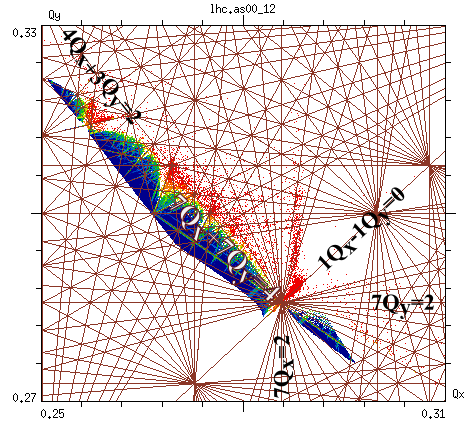
\includegraphics[width=1.0\linewidth]{2017injnocolc15o+19_6noerru_dp0_ord14_annotate_7th.png}
	\end{minipage}
	\begin{minipage}[t]{0.49\linewidth}
		\centering
		$7^{\mathrm{th}}$ H+V
		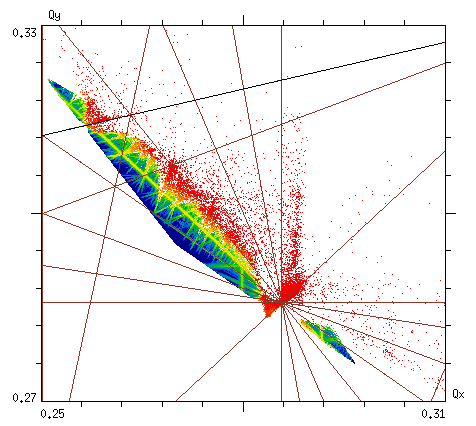
\includegraphics[width=1.0\linewidth]{2017injnocolc15o+19_6noerrut7skhv_dp0_ord7.png}
	\end{minipage}	
	\begin{minipage}[t]{0.49\linewidth}
		\centering
		$7^{\mathrm{th}}$ H
		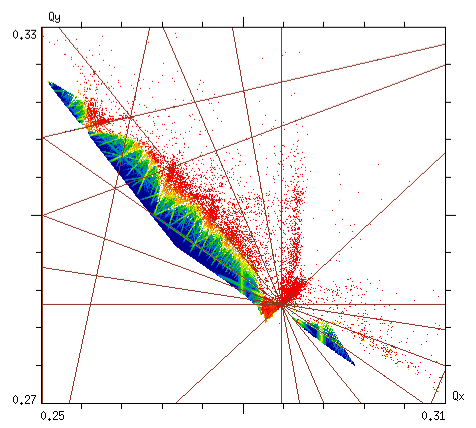
\includegraphics[width=1.0\linewidth]{2017injnocolc15o+19_6noerrut7skh_dp0_ord7.png}
	\end{minipage}
	\begin{minipage}[t]{0.49\linewidth}
		\centering
		$7^{\mathrm{th}}$ V
		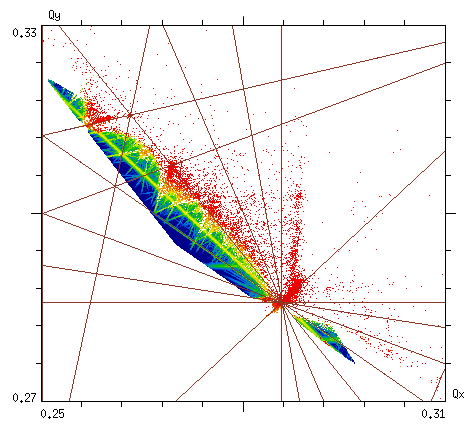
\includegraphics[width=1.0\linewidth]{2017injnocolc15o+19_6noerrut7skv_dp0_ord7.png}
	\end{minipage}	
	\caption{\label{fig:7th2017fma} FMA analysis in frequency space without excitation (top left) and for $7^{\mathrm{th}}$~turn pulsing in H+V (top right), only in H (bottom left) and only in V (bottom right) based on the 2017 injection optics with no machine errors and a tune of (62.27,60.295). The excitation is 96~nrad in both planes. The $7Q_x$ and $7Q_y$ resonance are both excited and in addition to the 14th order $7Q_x+7Q_y$.}
\end{figure*}

\begin{table}[b]
	\caption{\label{tab:7thexp}%
		Overview of the effect of $7^{\mathrm{th}}$~turn pulsing during the two resonant excitation experiments in 2016~\cite{resexmd2016} and 2017~\cite{resexmd2017}. The plane of the excitation is abbreviated with H for horizontal, V for vertical and H+V for horizontal and vertical at the same time.
	}
	\begin{ruledtabular}
		\begin{tabular}{lcc}
			Parameter & Experiment 2017 & Experiment 2016  \\
			\colrule
			optics & 2017 injection optics & 2016 injection optics \\
			tune $(Q_x,Q_y)$ & (62.27,60.295) & (64.28,59.31)\\\hline
			excitation plane  & H,V and H+V&  H\\
			losses & similar loss rates for  & large losses for \\
			& pulsing in H,V &  pulsing in H \\
			&  and H+V & \\
			hor. emit. growth & no & yes, very small \\
			vert. emit. growth & yes, for pulsing in & no\\
			&  V and H+V & \\
		\end{tabular}
	\end{ruledtabular}
\end{table}

\begin{figure*}[h]
	\begin{minipage}[t]{0.49\linewidth}
		\centering
		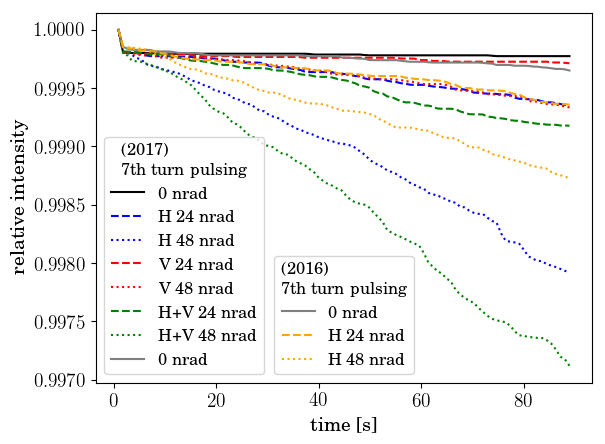
\includegraphics[width=1.0\linewidth]{2016+2017injerra2b2uran1_2e-3_7th_3_5um_intensity.png}
	\end{minipage}
	\begin{minipage}[t]{0.49\linewidth}
		\centering
		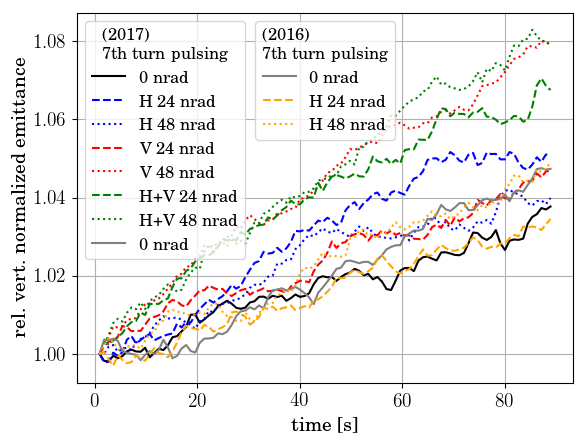
\includegraphics[width=1.0\linewidth]{2016+2017injerra2b2uran1_2e-3_7th_3_5um_rel_emit2.png}
	\end{minipage}
	\begin{minipage}[t]{0.49\linewidth}
		\centering
		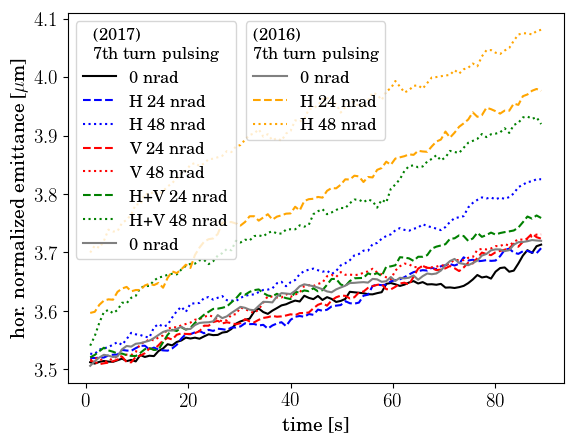
\includegraphics[width=1.0\linewidth]{2016+2017injerra2b2uran1_2e-3_7th_3_5um_emit1.png}
	\end{minipage}	
	\begin{minipage}[t]{0.49\linewidth}
		\centering
		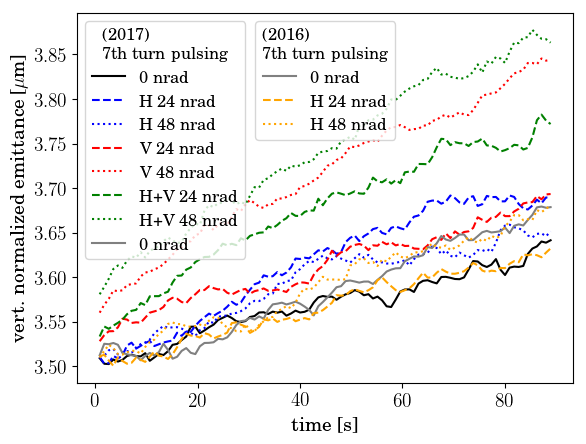
\includegraphics[width=1.0\linewidth]{2016+2017injerra2b2uran1_2e-3_7th_3_5um_emit2.png}
	\end{minipage}
	\caption{\label{fig:7thsim} Relative intensity (top left), relative vertical emittance (top right), and horizontal (bottom left) and vertical (bottom right) emittance obtained from distribution tracking based on the 2016 injection optics with standard errors and $(Q_x,Q_y)=(64.28,59.31)$ and 2017 injection optics with standard errors and $(Q_x,Q_y)=(62.27,60.295)$. The solid line indicates an excitation with only a random dipole noise component in H+V of 6~nrad, and the dotted and dashed line the results for $7^{\mathrm{th}}$~turn pulsing with two different excitation amplitudes plus a random dipole noise component in H+V of 6~nrad.}
\end{figure*}

The simulation results from the distribution tracking shown in Fig.~\ref{fig:7thsim} in general predict in terms of emittance for the two experiments:
\begin{description}
	\item[2016 experiment] Excitation amplitude dependent emittance growth in the horizontal but not in the vertical plane.
	\item[2017 experiment] Excitation amplitude dependent emittance growth in the vertical plane but not in the horizontal plane for an excitation in V and H+V. For an excitation only in H no emittance growth is observed.
\end{description}
Similar changes of the emittance as predicted in simulations were also experimentally observed as depicted in Fig.~\ref{fig:7thexp}, where emittance growth was observed only in the horizontal plane for pulsing in H in 2016, and only in the vertical plane for pulsing in V and H+V in 2017 with no emittance growth at all for pulsing in H. Just as for the $10^{\mathrm{th}}$~turn pulsing, the emittance growth can be divided also for the $7^{\mathrm{th}}$~turn pulsing in a phase of fast adjustment of the beam distribution and the reach of a new equilibrium state indicated in blue (fast adjustment) and black (equilibrium state) in Fig.~\ref{fig:7thexp}. Also in this case, the distribution changes are directly visible on the beam profiles taken with the BSRT (see Appendix~\ref{app:sec:7}, Fig.~\ref{fig:7thexpprof}).
\begin{figure*}[h]
		2016 experiment, $7^\mathrm{th}$ H	\\	\begin{minipage}[t]{0.32\linewidth}
		\centering
		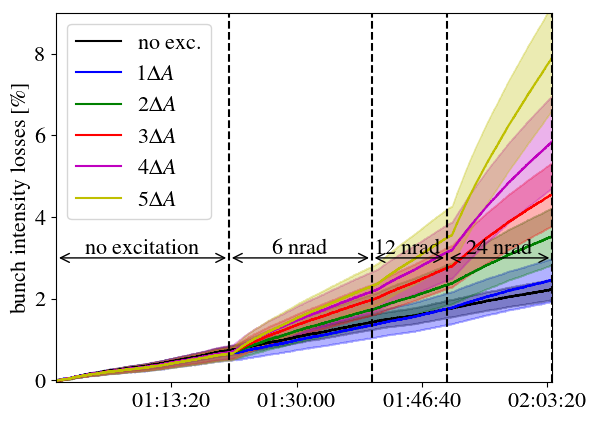
\includegraphics[height=0.75\linewidth]{2016_bunch_intensity_h7th_no_damper_avg.png}
	\end{minipage}	
	\begin{minipage}[t]{0.32\linewidth}
		\centering
		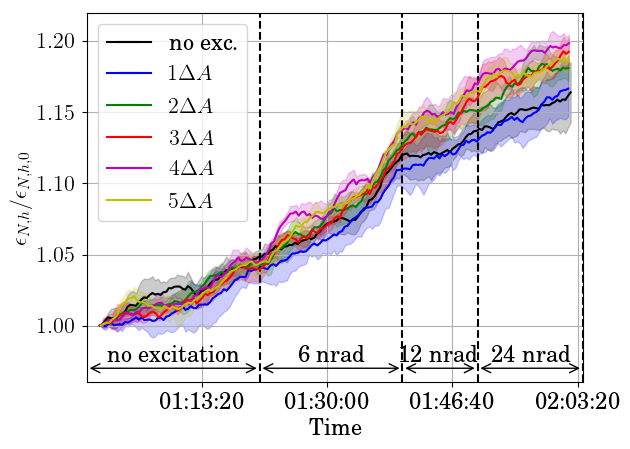
\includegraphics[height=0.75\linewidth]{2016_emith_avg_rel_h7th_no_damper.png}
	\end{minipage}	
	\begin{minipage}[t]{0.32\linewidth}
		\centering
		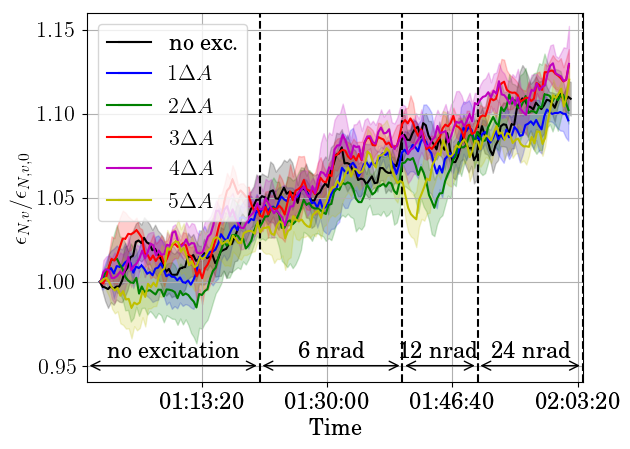
\includegraphics[height=0.75\linewidth]{2016_emitv_avg_rel_h7th_no_damper.png}
	\end{minipage}	
		2017 experiment, $7^\mathrm{th}$ H+V\\
	\begin{minipage}[t]{0.32\linewidth}
		\centering
		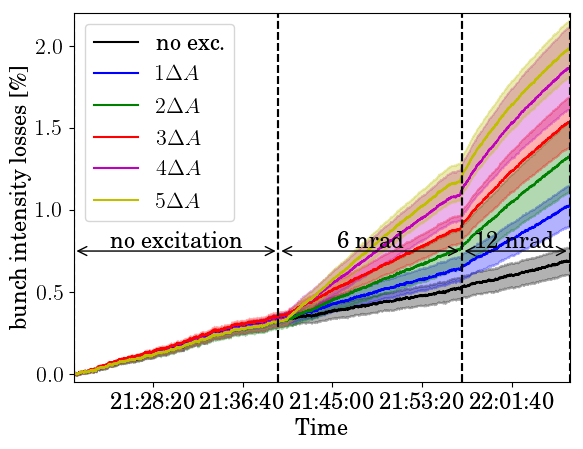
\includegraphics[height=0.75\linewidth]{2017_bunch_intensity_hv7th_no_damper_avg.png}
	\end{minipage}	
	\begin{minipage}[t]{0.32\linewidth}
		\centering
		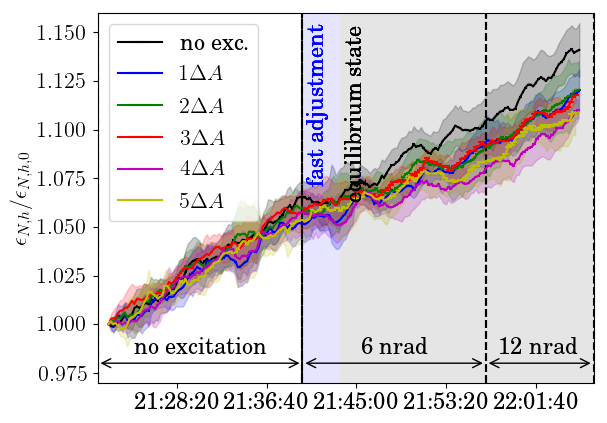
\includegraphics[height=0.75\linewidth]{2017_emith_avg_rel_hv7th_no_damper.png}
	\end{minipage}	
	\begin{minipage}[t]{0.32\linewidth}
		\centering
		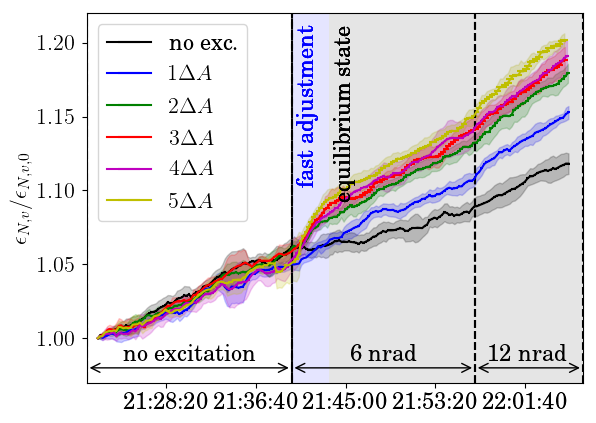
\includegraphics[height=0.75\linewidth]{2017_emitv_avg_rel_hv7th_no_damper.png}
	\end{minipage}	
	\caption{\label{fig:7thexp} Relative horizontal (top) and vertical (bottom) emittance obtained during the 2016 experiments (left) and the 2017 experiment (right) averaged over the bunches experiencing the same excitation amplitude. For all bunches the damper was not active.}
\end{figure*}

The losses measured during the experiment however differ from the simulations in terms of for which case the largest rate is observed as well as quantitatively for the specific cases. For example smaller losses are expected for the 2016 experiments compared to the 2017 experiments from simulations, while experimentally higher loss rates were measured in 2016 (see Fig.~\ref{fig:7thexploss}). For the 2017 experiment, the highest loss rates are expected for pulsing in H+V, than in H and then with a considerably reduction in V. During the experiment comparable loss rates are however measured for all three planes (see Appendix~\ref{app:sec:7}, Fig.~\ref{fig:7thexploss2017}). Last but not least the loss rates as defined in Eqn.~\ref{eqn:lossrate} for the 2016 (red and yellow) and 2017 (black and gree) experiments are compared in Fig.~\ref{fig:7thexploss}. In both cases and as also observed for the $10^{\mathrm{th}}$~turn pulsing, the loss rate follows a quadratic scaling with the excitation amplitude. Loss rates were in general higher during the 2016 experiments. The loss rates from simulations are not shown in Fig.~\ref{fig:7thexploss} as losses were only observed for much higher excitation amplitudes than tried in the experiments.
\begin{figure}[h]
	\centering
	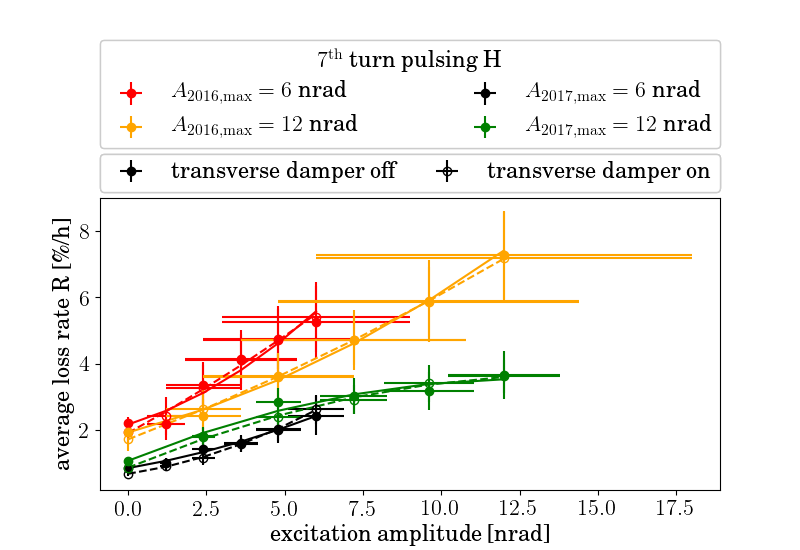
\includegraphics[width=1.0\linewidth]{2016+2017_scale_amp_7h_lblshort.png}
	\caption{\label{fig:7thexploss} Comparison of scaling of loss rates with excitation amplitude for $7^{\mathrm{th}}$~turn pulsing in H and data obtained during the 2016 experiment (black and blue) and 2017 experiment (red and yellow). The excitation amplitude error is 50\% in 2016 and was reduced to 15\% in 2017. The solid and dashed line indicate the second order polynomial fit to the loss rate.}
\end{figure}

\clearpage

\subsection{$8^{\mathrm{th}}$ turn pulsing\label{sec:simex8}}
Pulsing patterns which have little effect on the beam core are particularly interesting for the hollow electron lens operation if they in addition have a large effect on the halo. This is in general feasible considering the highly nonlinear field generated at the location of the halo particles by the HEL compared to no field or only a very small field at the location of the beam core. With this motivation in mind the $8^{\mathrm{th}}$~turn pulsing pattern was studied, for which a small effect in comparison to the $7^{\mathrm{th}}$ and $10^{\mathrm{th}}$ turn pulsing is expected (see Fig.~\ref{fig:8thsim}).
\begin{figure*}[h]
	\begin{minipage}[t]{0.49\linewidth}
		\centering
		\includegraphics[width=1.0\linewidth]{2017injerra2b2uran1_2e-3_8th_3_5um_intensity.png}
	\end{minipage}
	\begin{minipage}[t]{0.49\linewidth}
		\centering
		\includegraphics[width=1.0\linewidth]{2017injerra2b2uran1_2e-3_8th_3_5um_sigm.png}
	\end{minipage}
	\begin{minipage}[t]{0.49\linewidth}
		\centering
		\includegraphics[width=1.0\linewidth]{2017injerra2b2uran1_2e-3_8th_3_5um_emit1.png}
	\end{minipage}	
	\begin{minipage}[t]{0.49\linewidth}
		\centering
		\includegraphics[width=1.0\linewidth]{2017injerra2b2uran1_2e-3_8th_3_5um_emit2.png}
	\end{minipage}	
	\caption{\label{fig:8thsim} Relative intensity (top left), bunch length (top right), and horizontal (bottom left) and vertical (bottom right) emittance obtained from simulations (distribution tracking) based on the 2017 injection optics with standard errors and $(Q_x,Q_y)=(62.27,60.295)$. The solid line indicates an excitation with only a random dipole noise component in H+V of 6~nrad, and the dotted and dashed line the results for $8^{\mathrm{th}}$~turn pulsing plus a random dipole noise component in H+V of 6~nrad.}
\end{figure*}
\begin{figure*}[t]
	\begin{minipage}[t]{0.49\linewidth}
		\centering
		no excitation
		\includegraphics[width=1.0\linewidth]{2017injnocolc15o+19_6noerru_dp0_amp.png}
	\end{minipage}
	\begin{minipage}[t]{0.49\linewidth}
		\centering
		$8^{\mathrm{th}}$ H+V
		\includegraphics[width=1.0\linewidth]{2017injnocolc15o+19_6noerrut8skhv_dp0_amp_annotate.png}
	\end{minipage}	
	\caption{\label{fig:8th2017fmaamp} FMA analysis in amplitude space without excitation (left) and for $8^{\mathrm{th}}$~turn pulsing (right) based on the 2017 injection optics with no machine errors and a tune of (62.27,60.295). The excitation is 96~nrad in both planes. The $16Q_y$ and \mbox{$8Q_x-4Q_y$} are both excited.}
\end{figure*}
In simulations no visible effect is indeed observed for excitation amplitudes smaller than 96~nrad. In the horizontal and vertical plane a small emittance growth due to the excitation is visible, but without any clear dependence on the amplitude or plane. The FMA analysis in amplitude space reveals also the driven resonances (Fig.~\ref{fig:8th2017fmaamp}), which are the $16Q_y$ and \mbox{$8Q_x-4Q_y$} resonances and several even higher orders. These are in general very high order resonances whose effect is thus expected to be small.

\begin{figure}[h]
	\centering
	\includegraphics[width=1.0\linewidth]{2017_scale_amp_8hv_lblshort.png}
	\caption{\label{fig:8thexploss} Comparison of scaling of loss rates with excitation amplitude for $8^{\mathrm{th}}$~turn pulsing in H+V measured during the 2017 experiment. The excitation amplitude error is 15\% indicated by the horizontal error bars, the error on the loss rate is the error on the mean obtained through the average over the 6~bunches with the same excitation amplitude.}
\end{figure}
The small effect on the beam expected from simulations could then be also confirmed experimentally during the 2017 experiment. For this purpose the excitation amplitude was increased to the maximum reachable amplitude of 96~nrad. As depicted in Fig.~\ref{fig:8thexploss}, the loss rate increased slightly with the excitation amplitude for an excitation in H+V. For an excitation only in V or only in H, no statistically relevant increase was observed (see Appendix~\ref{app:sec:8}, Fig.~\ref{fig:8thexploss2017}). In the horizontal plane, a change in beam distribution was measured with the BSRT profiles (Appendix~\ref{app:sec:8}, Fig.~\ref{fig:8thexpprof}) for an excitation only in~H. The distribution increased around $2.0~\sigma$ simultaneously with a depletion of the beam core. For an excitation in H+V one would expect to see a similar distribution change. However, this change is not visible as the emittance of the references bunches was much smaller, around $1.8~\mu$m normalized emittance, compared to around $2.6~\mu$m for the excited bunches \cite{resexmd2017}. This difference in emittance then resulted in a stronger emittance growth due to intra-beam scattering for the reference bunches in comparison to the excited bunches making the additional emittance growth and distribution changes due to the excitation undetectable. In the vertical plane, the beam distribution and emittance were not affected by the resonant excitation.

\clearpage

\subsection{random excitation\label{sec:simexran}}
The random excitation presents in general the pulsing pattern leading to the fastest halo depletion rates achievable with an HEL. On the other hand this pattern is also the most dangerous one for the proton beam core. The aim of this experiment was to test the effect on the core in comparison to the resonant excitation represented in the 2017 experiment by primarily the $7^{\mathrm{th}}$~turn pulsing as for $8^{\mathrm{th}}$~turn pulsing basically no effect was observed. The random excitation is in general so powerful as it excites all frequencies of the beam equally.
\begin{figure*}[h]
	\begin{minipage}[t]{0.49\linewidth}
		\centering
		no excitation
		\includegraphics[width=1.0\linewidth]{2017injnocolc15o+19_6noerru_dp0_amp.png}
	\end{minipage}
	\begin{minipage}[t]{0.49\linewidth}
		\centering
		uniform random H+V
		\includegraphics[width=1.0\linewidth]{2017injnocolc15o+19_6noerruranadthv_1nrad_dp0_amp.png}
	\end{minipage}	
	\caption{\label{fig:ran2017fmaamp} FMA analysis in amplitude space without excitation (left) and for a uniform random excitation with 1~nrad amplitude (right) in H+V based on the 2017 injection optics with no machine errors and a tune of (62.27,60.295).}
\end{figure*}
This can be seen clearly on the example of the FMA analysis in amplitude space depicted in Fig.~\ref{fig:ran2017fmaamp}. In the case of a random excitation, the diffusion in tune is increased in comparison to the $k^{\mathrm{th}}$~turn pulsing rather equally for all particle amplitudes.
\begin{figure*}[h]
	\begin{minipage}[t]{0.49\linewidth}
		\centering
		\includegraphics[width=1.0\linewidth]{2017injerra2b2u_ranadt_3_5um_intensity.png}
	\end{minipage}
	\begin{minipage}[t]{0.49\linewidth}
		\centering
		\includegraphics[width=1.0\linewidth]{2017injerra2b2u_ranadt_3_5um_sigm.png}
	\end{minipage}
	\begin{minipage}[t]{0.49\linewidth}
		\centering
		\includegraphics[width=1.0\linewidth]{2017injerra2b2u_ranadt_3_5um_emit1.png}
	\end{minipage}	
	\begin{minipage}[t]{0.49\linewidth}
		\centering
		\includegraphics[width=1.0\linewidth]{2017injerra2b2u_ranadt_3_5um_emit2.png}
	\end{minipage}
	\caption{\label{fig:ransim} Relative intensity (top left), bunch length (top right), and horizontal (bottom left) and vertical (bottom right) emittance obtained from distribution tracking based on the 2017 injection optics with standard errors and $(Q_x,Q_y)=(62.27,60.295)$. The solid line indicates the case with no excitation, and the dotted and dashed line the results for a uniform random excitation of 12~nrad and 24~nrad respectively.}
\end{figure*}
The distribution tracking shown in Fig.~\ref{fig:ransim} also reveals a quite symmetric evolution of the beam parameters for a random excitation:
\begin{itemize}
	\item Emittance growth is only caused by an excitation in the same plane.
	\item The emittance growth is quantitatively comparable for an excitation in only the corresponding plane. Only a small increase or decrease is observed if the excitation is applied in both planes. The difference could be due to coupling.
	\item The random excitation leads to an increase of the emittance growth rate. Compared to the $k^{\mathrm{th}}$~turn pulsing there is explicitly no initial adjustment phase of the distribution.
	\item Negligible losses are observed independent of the plane of excitation.
\end{itemize}
\begin{figure*}[b]
	random excitation V\\
	\begin{minipage}[t]{0.32\linewidth}
		\centering
		\includegraphics[height=0.75\linewidth]{2017_bunch_intensity_vran_no_damper_avg.png}
	\end{minipage}	
	\begin{minipage}[t]{0.32\linewidth}
		\centering
		\includegraphics[height=0.75\linewidth]{2017_emith_avg_rel_vran_no_damper.png}
	\end{minipage}	
	\begin{minipage}[t]{0.32\linewidth}
		\centering
		\includegraphics[height=0.75\linewidth]{2017_emitv_avg_rel_vran_no_damper.png}
	\end{minipage}	
		random excitation H+V\\
	\begin{minipage}[t]{0.32\linewidth}
		\centering
		\includegraphics[height=0.75\linewidth]{2017_bunch_intensity_hvran_no_damper_avg.png}
	\end{minipage}	
	\begin{minipage}[t]{0.32\linewidth}
		\centering
		\includegraphics[height=0.75\linewidth]{2017_emith_avg_rel_hvran_no_damper.png}
	\end{minipage}	
	\begin{minipage}[t]{0.32\linewidth}
		\centering
		\includegraphics[height=0.75\linewidth]{2017_emitv_avg_rel_hvran_no_damper.png}
	\end{minipage}	
	\caption{\label{fig:ranexp} Relative intensity (left) and relative horizontal (center) and vertical (right) emittance for a random excitation only in V (top) and in H+V (bottom). Emittance growth is only caused in the plane of excitation.}
\end{figure*}

Qualitatively, this behavior could be also confirmed experimentally during the 2017 experiments. Here excitation amplitude dependent emittance growth was only recorded in the plane of excitation with all excitation amplitude dependent emittance growth rates in a comparable range. As example the relative horizontal and vertical emittance for pulsing in V and in H+V are depicted in Fig.~\ref{fig:ranexp}. Note that as expected from simulations and despite the large excitation amplitude dependent emittance growth, the growth rates stays constant. There is explicitly no fast adjustment phase succeeded by a new equilibrium state as observed for the $7^{\mathrm{th}}$ and $10^{\mathrm{th}}$~turn pulsing.
\begin{figure*}[h]
	\begin{minipage}[t]{0.49\linewidth}
		\centering
		reference bunch,\\ no excitation
		\includegraphics[width=1.0\linewidth]{profile_v_ranv_slot_1698.png}
	\end{minipage}
	\begin{minipage}[t]{0.49\linewidth}
		\centering
		excited bunch,\\ random excitation V
		\includegraphics[width=1.0\linewidth]{profile_v_ranv_slot_1532.png}
	\end{minipage}
	\caption{\label{fig:ranexpprof}Vertical beam profiles measured with the Beam Synchrotron Radiation Telescope (BSRT) during the 2017 experiments. The profiles are taken at the end of the random excitation in V. For both bunches the transverse damper is not active. The distribution changes in the reference bunch (left), here slot 1698, are much less than for the bunch experiencing the maximum excitation (right), here slot 2696.}
\end{figure*}
The changes in emittance are also directly visible in the beam profiles measured with the BSRT. As an example Fig.~\ref{fig:ranexpprof} shows the profile for a random excitation only in V in comparison to a reference bunch. The distribution also stays Gaussian in case of a random excitation in contrast to the $10^{\mathrm{th}}$~turn pulsing in which case it clearly assumes a non-Gaussian shape (see Fig.~\ref{fig:10thexpprof}).

\begin{figure*}[h]
	\begin{minipage}[t]{0.32\linewidth}
		\centering
		\includegraphics[width=1.0\linewidth]{2017_scale_amp_ranh_lblshort.png}
	\end{minipage}	
	\begin{minipage}[t]{0.32\linewidth}
		\centering
		\includegraphics[width=1.0\linewidth]{2017_scale_amp_ranv_lblshort.png}
	\end{minipage}	
	\begin{minipage}[t]{0.32\linewidth}
		\centering
		\includegraphics[width=1.0\linewidth]{2017_scale_amp_ranhv_lblshort.png}
	\end{minipage}	
	\caption{\label{fig:ranexplossplane} Comparison of scaling of loss rates with excitation amplitude for a random excitation only in H (top), only in V (center) and in H+V (bottom) measured during the 2017 experiment. The excitation amplitude error is 15\% indicated by the horizontal error bars. The loss rate is considerably reduced for the bunches with transverse damper active and is approximately additive with the excitation plane, meaning that double the loss rate is observed for an excitation in H+V compared to only in H or only in V.}
\end{figure*}
The experimental results for a maximum excitation amplitude of $A_{\mathrm{max}}=1$~nrad and $A_{\mathrm{max}}=6$~nrad also confirm the in general small losses predicted in simulations. The losses then increase more dramatically around the time when the maximum excitation amplitude is increased to $A_{\mathrm{max}}=12$~nrad (see Fig.~\ref{fig:ranexpprof}). This is most likely the point when, due to the large emittance growth, the physical aperture starts cutting into the more central region of the distribution. Furthermore, the dependence of the loss rate on the excitation plane is additive, meaning that double the loss rate is observed for an excitation in H+V compared to only in H or only V. The loss rate is also considerably reduced for the bunches with transverse damper active independent of the plane the excitation is applied in (see Fig.~\ref{fig:ranexplossplane}). In comparison to the $7^{\mathrm{th}}$~turn pulsing, the loss rate for a random excitation is smaller for a maximum excitation amplitude of $A_{\mathrm{max}}=6$~nrad, but larger for $A_{\mathrm{max}}=12$~nrad (see Fig.~\ref{fig:ranexploss}). This indicates an increase of the diffusion mostly in the beam tails for $7^{\mathrm{th}}$~turn pulsing, while for a random excitation mostly the core is affected.
\begin{figure}[h]
	\centering
	\includegraphics[width=1.0\linewidth]{2017_scale_amp_7th_ranhv_lblshort.png}
	\caption{\label{fig:ranexploss}  Comparison of scaling of loss rates with excitation amplitude for a random excitation and $7^{\mathrm{th}}$~turn pulsing in H+V measured during the 2017 experiment. The excitation amplitude error is 15\% indicated by the horizontal error bars.}
\end{figure}

\clearpage

\subsection{Effect of the transverse damper\label{sec:damp}}
\begin{figure*}[b]
	\centering
	damper not active\\
	\begin{minipage}[t]{0.32\linewidth}
		\centering
	random excitation V, 2017\\
		\includegraphics[height=0.75\linewidth]{2017_emitv_avg_rel_vran_no_damper.png}
	\end{minipage}	
	\begin{minipage}[t]{0.32\linewidth}
		\centering
		$7^{\mathrm{th}}$~turn V, 2017 exp.\\
		\includegraphics[height=0.75\linewidth]{2017_emitv_avg_rel_v7th_no_damper_no_text.png}
	\end{minipage}	
	\begin{minipage}[t]{0.32\linewidth}
		\centering
		$10^{\mathrm{th}}$~turn V, 2016 exp.\\
		\includegraphics[height=0.75\linewidth]{2016_emitv_avg_rel_v10th_no_damper_no_text.png}
	\end{minipage}	
	damper active\\
	\begin{minipage}[t]{0.32\linewidth}
		\centering
		random excitation V, 2017 exp.\\
		\includegraphics[height=0.75\linewidth]{2017_emitv_avg_rel_vran_with_damper.png}
	\end{minipage}	
	\begin{minipage}[t]{0.32\linewidth}
		\centering
		$7^{\mathrm{th}}$~turn V, 2017 exp.\\
		\includegraphics[height=0.75\linewidth]{2017_emitv_avg_rel_v7th_with_damper_no_text.png}
	\end{minipage}	
	\begin{minipage}[t]{0.32\linewidth}
		\centering
		$10^{\mathrm{th}}$~turn V, 2016 exp.\\
		\includegraphics[height=0.75\linewidth]{2016_emitv_avg_rel_v10th_with_damper_no_text.png}
	\end{minipage}	
	\caption{\label{fig:damp} Relative intensity for bunches with transverse damper not active (top) and transverse damper active (bottom) for a random excitation only in V (left) and for $7^{\mathrm{th}}$ (center) and $10^{\mathrm{th}}$~turn pulsing only in V (right).}
\end{figure*}
For all $k^{\mathrm{th}}$~turn pulsing patterns tested experimentally, the transverse damper does in general not change any of the observables studied during the experiments, explicitly losses, emittance and beam distribution suggesting that indeed it is not damping any resonant excitation. On the other hand, the transverse damper considerably decreases any changes of the above parameters in case of a random excitation. As an example, the vertical emittance growth for the $7^{\mathrm{th}}$ and $10^{\mathrm{th}}$~turn pulsing in V is compared with a random excitation in V in Fig.~\ref{fig:damp}. The same observation is also made in case of losses as shown in Fig.~\ref{fig:ranexploss} comparing the $7^{\mathrm{th}}$~turn pulsing in H+V with a random excitation in H+V. For the $7^{\mathrm{th}}$~turn pulsing the two curves for the transverse damper active and not active almost coincide while for the random excitation a significant difference is visible. Until present, it is unknown why the transverse damper (ADT) appears to be incapable of damping any resonant excitation as it fulfills all requirements to detect as well as damp the caused oscillation:
\begin{itemize}
	\item The closed orbit distortion caused by the resonant excitation during the experiments is large enough to be detectable with the ADT pickups.
	\item The ADT compares the position of each bunch with its position in the previous turn in order to detect an orbit distortion to be damped. Therefore an oscillation due to any $k^{\mathrm{th}}$~turn pulsing with $k>1$ would be noticed and damped.
	\item The ADT is capable of damping the oscillation of each bunch individually. The ADT should therefore be capable of applying the correct corrective kick for each group of bunches seeing the same excitation amplitude.
\end{itemize}
Further studies are therefore needed in order to obtain a deeper understanding of the interaction of the transverse damper with a resonant excitation.
\clearpage

\section{Summary\label{sec:sum}}
This paper intends to give an overview of the effects of the hollow electron lens (HEL) on the proton beam core and the experiments conducted in this context at the LHC in 2016~\cite{resexmd2016} and 2017~\cite{resexmd2017}. For a perfect HEL without any imperfections no effect on the core is to be expected as the field at the center vanishes by construction. Only in the case of imperfections in the guidance and profile of the electron beam, a residual kick on the proton beam core can occur. In this case and assuming HL-LHC parameters (Tables~\ref{tab:hllhc_param}--\ref{tab:hel_param}), the contribution from the electron lens bends with approximately $0.5$~nrad to first order is negligible with respect to the kick expected from the central region of the HEL of approximatley $20$~nrad to first order caused by profile imperfections in the electron beam. In DC operation these kicks, even if nonlinear in reality, are negligible compared to the nonlinearities present in the LHC and HL-LHC and are thus of no concern. The picture changes if the HEL is operated in pulsed mode, in which case noise is introduced on the halo particles (intended) as well as on the beam core (unintended) in the presence of imperfections of the HEL entailing much more stringent tolerances.

To study the effect on the beam core in case of the much more dangerous pulsed operation, beam experiments were conducted in 2016 and 2017 at injection. As no hollow electron lens is currently installed in the LHC, the in reality non-linear kick was emulated to first order by a dipole kick with the corresponding excitation pattern. The experimental results in general suggest that for the kick amplitudes as expected from the HEL, considerable effects are to be expected for a random excitation and certain resonant excitations, explicitly $7^{\mathrm{th}}$ and $10^{\mathrm{th}}$~turn pulsing during the conducted experiments. In addition, also one resonant excitation pattern, the $8^{\mathrm{th}}$~turn pulsing, was tested featuring a small effect on the beam core. Assuming that this pattern has a large effect on the beam halo, it would be an optimal candidate for a feasible HEL excitation pattern.

The resonant excitation in general features a rich nonlinear dynamics leading to a diversity in beam distribution and diffusion changes as can be seen for example from the very diverse effects of the different $k^{\mathrm{th}}$~turn pulsing patterns observed in simulations and experiments. The origin of this diversity is due to the fact that only certain frequencies and thus resonances are excited. Typical for the resonant excitation is also the fast adjustment of the beam distribution to a new equilibrium state which could be for the first time measured in the experiments and predicted in the simulations presented in this paper. The random excitation on the other hand excites all beam frequencies equally, leading to the highest increase in halo removal rates for the HEL \cite{hel_halo_hllhc_fitterer} but also the strongest effects on the core, mainly in terms of strong emittance growth as predicted in simulations, experiments and also a multitude of earlier publications on the subject of random noise. From the experiments the tolerances summarized in Table~\ref{tab:tolexp} could be obtained, where for each excitation pattern and plane the smallest kick amplitude is listed for which an increase in emittance or losses was observed.
\begin{table}
	\caption{\label{tab:tolexp}%
		Minimum kick amplitudes $\Delta z'$ for which either an increase in emittance or losses was observed during the LHC experiments. The tolerances are given for the case of the transverse damper not active. The same tolerances are obtained for the case with the damper active in case of all resonant excitation. In case of a random excitation the tolerance can be increased by roughly a factor~2.
	}
	\begin{ruledtabular}
		\begin{tabular}{lccc}
		pulsing pattern & exp. year & plane & $\Delta z' \ [\mathrm{nrad}]$  \\
			\colrule
			random & 2017 & H or V & 2.4 \\
			 & & H+V & 1.2 \\\hline
			$7^{\mathrm{th}}$~turn & 2016 & H & 2.4 \\
			 & 2017 & H & 2.4 \\
			 & 2017 & V & 1.2 \\
			 & 2017 & H+V & 1.2 \\\hline
			$8^{\mathrm{th}}$~turn & 2017 & H & 14.4 \\
			& 2017 & V & $>96$ \\
			& 2017 & H+V & 12 \\\hline
			$10^{\mathrm{th}}$~turn & 2016 & V & 9.6 \\
		\end{tabular}
	\end{ruledtabular}
\end{table}
Tolerances in case of a random excitation are extremely stringent. For a resonant excitation the effect depends strongly on the order $k$ of the $k^{\mathrm{th}}$~turn pulsing. For a future HEL, the pattern could therefore be tuned to the machine and beam configuration in order to yield a strong effect on the halo particles and small effect on the beam core. Compared to the estimated kick amplitude of the HEL on the beam core of
\begin{equation}
\Delta x', \Delta y' = 20 \ \mathrm{nrad}
\end{equation}
the tolerances for all experimentally tried pulsing pattern except for $8^{\mathrm{th}}$~turn pulsing in V lie below this value. As a next step, the experiment should be conducted at collision energy where the HEL is most needed. At collision energy the inherent noise level of the LHC is smaller which could lead to more relaxed tolerances than the ones obtained at injection energy.



\begin{acknowledgments}
We wish to acknowledge Giulia Papotti with her help with the preparations for the 2016 experiments and her general support from the operations side, Roderik Bruce and Gianluca Valentino for there very helpful suggestions in preparing the experiment at the LHC and we would like to thank all participants of the experiment for helping acquire the data presented in this paper. We wish to thank Sergei Nagaitsev for the very useful discussion and profound question to find out why the transverse damper is not damping any resonant excitation. We would like to acknowledge Dmitry Shatilov for his help with the Lifetrac code, and St\'{e}phane Fartoukh, Riccardo De Maria and Rogelio Tomás for their help with generating the appropiate optics model. We are grateful also for the support from the beam instrumentation team, in particular Enrico Bravin and Georges Trad, with the BSRT and are thankful for the collaboration with St\'{e}phania Papadopoulou and Fanouria Antonio for the analysis of the BSRT profiles.
\end{acknowledgments}

\newpage

\appendix
\section{Additional plots for 10th turn pulsing during the 2016 experiments}
\label{app:sec:10}
\begin{figure}[h]
	\begin{minipage}[t]{0.49\linewidth}
		\centering
		no excitation
		\includegraphics[width=1.0\linewidth]{2016injnocolc15o+19_6noerru_dp0_ord10_annotate.png}
	\end{minipage}
	\begin{minipage}[t]{0.49\linewidth}
		\centering
		$10^{\mathrm{th}}$ H+V
		\includegraphics[width=1.0\linewidth]{2016injnocolc15o+19_6noerrut10skhv_dp0_ord10.png}
	\end{minipage}	
	\begin{minipage}[t]{0.49\linewidth}
		\centering
		$10^{\mathrm{th}}$ H
		\includegraphics[width=1.0\linewidth]{2016injnocolc15o+19_6noerrut10skh_dp0_ord10.png}
	\end{minipage}	
	\begin{minipage}[t]{0.49\linewidth}
		\centering
		$10^{\mathrm{th}}$ V
		\includegraphics[width=1.0\linewidth]{2016injnocolc15o+19_6noerrut10skv_dp0_ord10.png}
	\end{minipage}
	\caption{\label{app:fig:fma:10} FMA analysis for $10^{\mathrm{th}}$~turn pulsing based on the 2016 injection optics with no machine errors and a tune of (64.28,59.31). The excitation is 120~nrad in the corresponding plane. There is no significant difference in the FMA analysis between pulsing only in H, only in V or in H+V.}
\end{figure}

\newpage

\section{Additional plots for $7^{\mathrm{th}}$~turn pulsing during 2017 experiments}
\label{app:sec:7}
\begin{figure}[h]
	\begin{minipage}[t]{1.0\linewidth}
	\centering
	\includegraphics[width=0.9\linewidth]{2017_scale_amp_7h_lblshort.png}
	\end{minipage}
	\begin{minipage}[t]{1.0\linewidth}
		\centering
		\includegraphics[width=0.9\linewidth]{2017_scale_amp_7v_lblshort.png}
	\end{minipage}
	\begin{minipage}[t]{1.0\linewidth}
		\centering
		\includegraphics[width=0.9\linewidth]{2017_scale_amp_7hv_lblshort.png}
	\end{minipage}
	\caption{\label{fig:7thexploss2017} Comparison of scaling of loss rates with excitation amplitude for $7^{\mathrm{th}}$~turn pulsing only in H (top), only in V (center) and in H+V (bottom) during the 2017 experiment. The excitation amplitude error is 15\% indicated by horizontal error bars. The vertical errorbars represent the pure statistical error based on the averaging over several bunches with the same excitation amplitude.}
\end{figure}
\begin{figure}[h]
	\begin{minipage}[t]{0.49\linewidth}
		\centering
		reference bunch,\\ no excitation
		\includegraphics[width=1.0\linewidth]{profile_v_7thhv_slot_2862.png}
	\end{minipage}
	\begin{minipage}[t]{0.49\linewidth}
		\centering
		excited bunch,\\ $7^{\mathrm{th}}$~turn H+V	
		\includegraphics[width=1.0\linewidth]{profile_v_7thhv_slot_2696.png}
	\end{minipage}
	\caption{\label{fig:7thexpprof} Vertical beam profiles measured with the Beam Synchrotron Radiation Telescope (BSRT) during the 2017 experiments. The profiles are taken at the end of the $7^{\mathrm{th}}$~turn pulsing in H+V. For both bunches the transverse damper is not active. The distribution changes in the reference bunch (left), here slot 2862, are much less than for the bunch experiencing the maximum excitation (right), here slot 2696.}
\end{figure}

\newpage

\section{Additional plots for $8^{\mathrm{th}}$~turn pulsing during 2017 experiments}
\label{app:sec:8}
\begin{figure}[h]
	\begin{minipage}[t]{1.0\linewidth}
		\centering
		\includegraphics[width=0.9\linewidth]{2017_scale_amp_8h_lblshort.png}
	\end{minipage}
	\begin{minipage}[t]{1.0\linewidth}
		\centering
		\includegraphics[width=0.9\linewidth]{2017_scale_amp_8v_lblshort.png}
	\end{minipage}
	\begin{minipage}[t]{1.0\linewidth}
		\centering
		\includegraphics[width=0.9\linewidth]{2017_scale_amp_8hv_lblshort.png}
	\end{minipage}
	\caption{\label{fig:8thexploss2017} Comparison of scaling of loss rates with excitation amplitude for $8^{\mathrm{th}}$~turn pulsing only in H (top), only in V (center) and in H+V (bottom) during the 2017 experiment. The excitation amplitude error is 15\% indicated by horizontal error bars. The vertical errorbars represent the pure statistical error based on the averaging over several bunches with the same excitation amplitude.}
\end{figure}
\begin{figure}[h]
	\begin{minipage}[t]{0.49\linewidth}
		\centering
		reference bunch,\\ no excitation
		\includegraphics[width=1.0\linewidth]{profile_h_8thh_slot_804.png}
	\end{minipage}
	\begin{minipage}[t]{0.49\linewidth}
		\centering
		excited bunch,\\ $8^{\mathrm{th}}$~turn H
		\includegraphics[width=1.0\linewidth]{profile_h_8thh_slot_632.png}
	\end{minipage}
	\caption{\label{fig:8thexpprof} Horizontal beam profiles measured with the Beam Synchrotron Radiation Telescope (BSRT) during the 2017 experiments. The profiles are taken at the end of the $8^{\mathrm{th}}$~turn pulsing in H. For both bunches the transverse damper is not active. The distribution changes in the reference bunch (left), here slot 804, are much less than for the bunch experiencing the maximum excitation (right), here slot 632.}
\end{figure}

\clearpage

\bibliography{resex-bibdesk}

\end{document}
